\documentclass[lang=cn,newtx,10pt,scheme=chinese]{elegantbook}

\title{计算语言学中的数学方法}
\subtitle{2023级用}

\author{王予沛 \& \texttt{ChatGPT}}
\institute{北京师范大学中文信息处理研究所}
% \date{2022/12/31}
% \version{4.5}
% \bioinfo{自定义}{信息}

\extrainfo{
% 本讲义扩展自\href{https://github.com/afshinea/stanford-cs-229-machine-learning}{斯坦福大学CS229小抄}\\
封面图片由\href{https://www.midjourney.com/home/}{Midjourney}创作
}

\setcounter{tocdepth}{3}

\logo{logo-blue.png}
\cover{cover_0913.png}

% 本文档命令
\usepackage{array}
\usepackage{arydshln}
\newcommand{\ccr}[1]{\makecell{{\color{#1}\rule{1cm}{1cm}}}}

% 修改标题页的橙色带
\definecolor{customcolor}{RGB}{32,178,170}
\colorlet{coverlinecolor}{customcolor}
\usepackage{cprotect}
\usepackage{amsmath}
\usepackage{blindtext}
\usepackage{hyperref}

\definecolor{mygray}{gray}{0.9}
\definecolor{headergray}{gray}{0.7}

% Define custom colors
\definecolor{myred}{rgb}{0.8, 0.2, 0.2}
\definecolor{myblue}{rgb}{0.2, 0.2, 0.8}
\definecolor{mygreen}{rgb}{0.0, 0.5, 0.0}
\definecolor{myorange}{rgb}{1.0, 0.5, 0.0}
\definecolor{mybrown}{rgb}{0.6, 0.4, 0.2}
\definecolor{mypurple}{rgb}{0.6, 0.2, 0.6}

\addbibresource[location=local]{reference.bib} % 参考文献,不要删除

\begin{document}

\maketitle
\frontmatter

\tableofcontents

\mainmatter

\chapter{矩阵与变换}

\begin{introduction}
  \item 从方程组到矩阵
  \item 从线性变换到矩阵
  \item 矩阵的运算
  \item 矩阵的性质
\end{introduction}

参考资料:
\begin{enumerate}
    \item \href{https://github.com/afshinea/stanford-cs-229-machine-learning/blob/master/zh/refresher-algebra-calculus.pdf}{Machine Learning cheatsheets for Stanford's CS 229 - VIP Refresher: Linear Algebra and Calculus};
    \item \href{https://math.mit.edu/~gs/linearalgebra/ila5/indexila5.html}{Introduction to Linear Algebra, Fifth Edition (2016)};
    \item 高中数学人教A版选修4-2:矩阵与变换.
\end{enumerate}

%%%%%%%%%%%%%%%%%%%%%%%%%%%%%%%%%%%%%%%%%%%
\section{从方程组到矩阵}
\label{sec:origin_of_matrix}

\begin{note}
本节旨在帮助学生了解矩阵产生的原因,它源于人们在解方程组时对简洁表达的需求。
\end{note}

\subsection{二元一次方程组}
\label{subsec:二元一次方程组}

让我们首先回顾一下二元一次方程组的基本概念。一个二元一次方程组由两个含有两个变量的一次方程组成。一般形式如下:

\begin{equation}
\left\{
\begin{array}{l}
ax_1 + bx_2 = c\\
dx_1 + ex_2 = f
\end{array}
\right.
\label{eq:二元一次方程组通式}
\end{equation}

其中,\(x_1\) 和 \(x_2\) 是我们要找的未知数,而 \(a\)、\(b\)、\(c\)、\(d\)、\(e\) 和 \(f\) 是已知的常数。

要解这样的方程组,我们通常会使用以下两种方法之一:
\begin{enumerate}
    \item \textbf{代数方法}:这种方法包括“代入法”和“消元法”。
    \begin{enumerate}
        \item 在代入法中,我们从一个方程中解出一个变量的表达式,然后将其代入另一个方程;
        \item 在消元法中,我们通过加减两个方程来消除一个变量,从而找到另一个变量的值。
    \end{enumerate}
    \item \textbf{图形方法}:在这种方法中,我们将每个方程视为二维空间中的一条直线。方程组的解就是这两条直线的交点。
\end{enumerate}


下面,我们使用\textbf{消元法}来解以下二元一次方程组:

\begin{equation}
    \left\{
        \begin{array}{l}
        2x_1 + 3x_2 = 5\\
        4x_1 + 5x_2 = 7
        \end{array}
        \right.
\label{eq:二元一次方程组示例}
\end{equation}

我们的目标是找到满足这两个方程的\(x_1\)和\(x_2\)的值。我们可以通过以下步骤来实现这一目标:

\begin{enumerate}
    \item 首先,我们可以使用第一个方程来消去第二个方程中的\(x_1\)。为此,我们可以将第一个方程的两边都乘以2,得到新的方程:
    \[
    4x_1 + 6x_2 = 10
    \]
    \item 接着,我们将新得到的方程从第二个方程中减去,从而消去\(x_1\):
    \[
    4x_1 + 5x_2 - (4x_1 + 6x_2) = 7 - 10
    \]
    这将给我们一个只包含\(x_2\)的方程:
    \[
    -x_2 = -3
    \]
    从中我们可以找到\(x_2\)的值:
    \[
    x_2 = 3
    \]
    \item 事实上,\(x_2 = 3\)可以看成一个方程,我们可以使用它来消去第一个方程中的\(x_2\):
    \[
    (2x_1 + 3x_2) + (-3) \cdot x_2 = 5 + (-3) \cdot 3
    \]
    这将给我们:
    \[
    2x_1 = 5 - 9
    \]
    从中我们可以找到\(x_1\)的值:
    \[
    2x_1 = -4
    \]
    \[
    x_1 = -2
    \]
\end{enumerate}

所以,该方程组的解是:
\[
x_1 = -2, \quad x_2 = 3
\]


在下一节中,我们将介绍如何使用高斯消元法和矩阵来更简洁地表达求解过程。

\vspace{0.5cm}

\begin{note}
    用方程$u$减去方程$v$指:用方程$u$的左边减去方程$v$的左边,用方程$u$的右边减去方程$v$的右边。
\end{note}

\subsection{系数矩阵和增广矩阵}
\label{subsec:系数矩阵和增广矩阵}

考虑二元一次方程组(\ref{eq:二元一次方程组示例})。
我们将方程组中方程的所有系数按照它们在整理好的方程中的位置取出来写成如式\ref{eq:系数矩阵示例}的一张数表。
有了这张数表我们就可以更加简洁地表达方程组中未知数的系数,
因此我们将其称为方程组的\textcolor{third}{\bf 系数矩阵},我们将其记为大写字母$A$。
由于矩阵$A$的尺寸是$2\times 2$,因此我们称其为$2\times 2$矩阵,或者$2$阶(方形)矩阵。

\begin{equation}
  A = \left(\begin{array}{ll}
2 & 3 \\
4 & 5
\end{array}\right)
\label{eq:系数矩阵示例}
\end{equation}

如果我们在系数矩阵右边增加一列$c$,用于记录方程的右端项(right hand side, RHS),则方程组(\ref{eq:二元一次方程组示例})可以写作$Ax=c$。我们用一根竖线隔开表示系数的数表和表示右端项的数列,得到的整个新数表称为方程组\ref{eq:二元一次方程组示例}的\textcolor{third}{\bf 增广矩阵},如式\ref{eq:增广矩阵示例}所示:
\begin{equation}
    [A \mid c]=\left(\begin{array}{cc|c}
2 & 3 & 5 \\
4 & 5 & 7
\end{array}\right)
\label{eq:增广矩阵示例}
\end{equation}

下面,我们对增广矩阵实施第\ref{subsec:二元一次方程组}节中所使用的消元法,从而达到解方程的目的:

\begin{enumerate}
    \item 首先,我们用第一行的系数来将第二行的系数化为$0$,具体操作如下:
    \begin{enumerate}
        \item 用第二行的第一个系数$4$除以第一行的第一个系数$2$,得到商数$2$;
        \item 将第一行整体乘以此商数($2$),得到$(4,6,10)$;
        \item 再用第二行减去第一行,则第二行的第一个元素变为$0$。这时增广矩阵变为:
        \begin{equation}
            \left(\begin{array}{cc|c}
        2 & 3 & 5 \\
        0 & -1 & -3
        \end{array}\right)
        \label{eq:行阶梯形矩阵}
        \end{equation}
        \item 在第二行两边乘以$-1$
    \end{enumerate}
    \item 现在用第二行中$x_2$的系数来将第一行中$x_2$的系数化为$0$,具体操作如下:
    \begin{enumerate}
        \item 用第一行的第二个系数$3$除以第二行的第二个系数$1$,得到商数$3$;
        \item 将第二行整体乘以此商数($3$),得到$(0,3,9)$;
        \item 再用第一行减去第二行,则第一行的第二个元素变为$0$。这时增广矩阵变为:
        \[
        \left(\begin{array}{cc|c}
        2 & 0 & -4 \\
        0 & 1 & 3
        \end{array}\right)
        \]
        \item 在第一行两边乘以$\frac{1}{2}$,得到增广矩阵:
        \begin{equation}
            \left(\begin{array}{cc|c}
        1 & 0 & -2 \\
        0 & 1 & 3
        \end{array}\right)
        \label{eq:简化行阶梯形矩阵}
        \end{equation}
    \end{enumerate}
\end{enumerate}

该式还原为方程组为

\[
\left\{
\begin{array}{l}
1 \cdot x_1 + 0 \cdot x_2 = -2\\
0 \cdot x_1 + 1\cdot x_2 = 3
\end{array}
\right.
\]


最终得到$x_1=-2$,$x_2=3$,这就是原方程组的解。

矩阵提供了一种组织方程组系数和常数项的方式,通过矩阵运算可以方便地求解方程组。这启发了矩阵理论的产生和发展。


\subsection{高斯-若尔当消元法}
\label{subsec:高斯-若尔当消元法}

回顾我们在第\ref{subsec:系数矩阵和增广矩阵}节中的操作,我们在增广矩阵上进行消元法时,仅仅使用了两种操作:
\begin{itemize}
    \item 把某行乘以一非零常数;
    \item 把第 $i$ 行加上第 $j$ 行的 $k$ 倍;
\end{itemize}

可见这些操作都是对矩阵的“行”进行的,因此我们称它们为\textcolor{third}{\bf 行变换}。

注意到,在进行消元法的过程中,我们得到的增广矩阵\ref{eq:行阶梯形矩阵}的非零元素看起来像是一个“倒过来的楼梯”,其第一行左起第一个非零元下方都是零,第二行左起第一个非零元在第一行左起第一个非零元的右侧,我们称这样的矩阵是\textcolor{third}{\bf 行阶梯形矩阵}。

\begin{definition}[行阶梯形矩阵]
    如果一个矩阵满足下面的条件,我们称其为{\bf 行阶梯形矩阵}(Row Echelon Form):
    \begin{enumerate}
        \item 所有仅包含零的行都位于矩阵的最底部;
        \item 在每一个非零行中,最左边的非零元素(称主元)总是出现在上一行主元的右侧;
        \item *包含非零元素的行中,首个非零元素必须为$1$.
    \end{enumerate}
    其中第三个条件是可选的,不同文献中有不同的定义方式,不必纠结。
\end{definition}

事实上,得到增广矩阵\ref{eq:行阶梯形矩阵}后,我们已经不再需要继续消元了。从第二行我们可以很容易的得到$-x_2=-3$,从而解出$x_2=3$。从第一行我们得到方程$2x_1+3x_2=5$,这时候我们使用\textbf{回代法},将$x_2=3$代到方程$2x_1+3x_2=5$中得到$2x_1+3\cdot 3=5$,从而解出$x_1=-2$。

一般地,我们称\textcolor{second}{“先通过行变换将矩阵化为行阶梯矩阵,然后直接通过回代法找到方程组的解”}这样的解方程的方法为\textcolor{third}{\bf 高斯消元法}。可以证明,任何矩阵都可以通过高斯消元法转换为简化行阶梯形形式

此外,当消元法进行到尾声时,我们得到的增广矩阵\ref{eq:简化行阶梯形矩阵}非常有特点,其每一行的第一个非零元素全是$1$,且这些行的第一个元素$1$所在列的其余元素全为零,我们称这样的矩阵是\textcolor{third}{\bf 简化行阶梯形矩阵}。显然,根据简化行阶梯形矩阵我们很容易得到方程组的解。

\begin{definition}[简化行阶梯形]
    如果一个矩阵满足下面的条件,我们称其为{\bf 简化行阶梯形}(Reduced Row Echelon Form, RREF):
\begin{enumerate}
    \item 所有零行都位于矩阵的底部;
    \item 在每一个非零行中,第一个非零元素(称主元)总是出现在上一行主元的右侧;
    \item 每一个非零行的主元都是$1$;
    \item \textcolor{red}{一个主元所在的列的其他元素都是$0$}。
\end{enumerate}

简化行阶梯形和行阶梯形矩阵的主要区别在于最后一条。

\end{definition}

一般地,我们称\textcolor{second}{“先通过行变换将矩阵化为行阶梯矩阵,然后进一步做行变换,将其化为简化行阶梯形矩阵进而直接\textbf{读出}方程组的解”}这样的解方程的方法为\textcolor{third}{\bf 高斯-若尔当消元法}。可以证明,任何矩阵都可以通过高斯-若尔当消元法转换为简化行阶梯形形式。高斯-若尔当消元法实际上是高斯消元法的一个扩展。

\subsection{矩阵的行列式}

\begin{note}
    行列式来自于数学家们在求解方程组时发现的一个可以用来简化表达,并判断方程组是否有解的记号。
\end{note}

\vspace*{0.3cm}

考虑二元一次    方程组(\ref{eq:二元一次方程组通式}),我们使用高斯-若尔当消元法求出该方程的解。
\begin{equation*}
\left[
\begin{array}{cc|c}
a & b & c \\
d & e & f
\end{array}
\right]
\xrightarrow{}
    \left[
    \begin{array}{cc|c}
1 & \frac{b}{a} & \frac{c}{a} \\
0 & e - \frac{bd}{a} & f - \frac{cd}{a}
\end{array}
\right]
\xrightarrow{}
\left[
\begin{array}{cc|c}
1 & 0 & \frac{ce - bf}{ae - bd} \\
0 & 1 & \frac{af - cd}{ae - bd}
\end{array}
\right]
\end{equation*}

如果我们定义$D=ae - bd, D_1=ce-bf, D_2=af - cd$,我们可以将原方程的结果表示为:
\begin{equation}
x_1 = \frac{D_1}{D},\quad x_2 = \frac{D_2}{D}
\end{equation}

这个结果称为二元一次方程组的\textcolor{third}{\bf 克莱姆法则}(Cramer's Rule)。其中$D$称为矩阵
$
\begin{bmatrix}
a & b \\
d & e
\end{bmatrix}
$
的行列式,记作
\begin{equation}
D = \operatorname*{det} \left(
    \begin{bmatrix}
        a & b \\
        d & e
        \end{bmatrix}
\right) = 
\left|
    \begin{array}{cc}
    a & b \\
    d & e
    \end{array}
\right|
= ae - bd
\end{equation}

同理有,

\begin{equation}
    D_1 = \operatorname*{det} \left(
        \begin{bmatrix}
            c & b \\
            f & e
            \end{bmatrix}
    \right) = 
    \left|
        \begin{array}{cc}
            c & b \\
            f & e
        \end{array}
    \right| = ce-bf, \quad
    D_2 = \operatorname*{det} \left(
        \begin{bmatrix}
            a & c \\
            d & f
            \end{bmatrix}
    \right) = 
    \left|
        \begin{array}{cc}
        a & c \\
        d & f
        \end{array}
    \right| = af - cd
\end{equation}

考虑一个特殊的方程组
\begin{equation}
    \left\{
        \begin{array}{l}
        x_1 + x_2 = 5\\
        x_1 + x_2 = 7
        \end{array}
        \right.
\end{equation}

显然,该方程组无解,其中$D=0$。可见,凡是系数矩阵的行列式$D=0$的二元一次方程组都是无解的。


一般地,考虑任意$n$元一次方程组(矩阵表示):
\begin{equation}
    A x=c
\label{eq:一般方程组的矩阵形式}
\end{equation}

其中的 $A$ 是一个 $n \times n$ 的方阵, 而向量 $x=\left(x_1, x_2, \cdots x_n\right)^T$和$c=\left(c_1, c_2, \cdots c_n\right)^T$ 均为长度为 $n$ 的列向量。 

克莱姆法则说明: 如果 $\operatorname{det} A \neq 0$ ,那么方程(\ref{eq:一般方程组的矩阵形式})有解$x=\left(x_1, x_2, \cdots x_n\right)^T$,其中

$$
x_i=\frac{\operatorname{det}\left(A_i\right)}{\operatorname{det}(A)}
$$

当中 $x_i$ 是列向量 $x$ 的第 $i$ 行,$A_i$ 是用列向量 $c$ 取代 $A$ 的第 $i$ 列后得到的矩阵。

注意到,我们仅定义了二阶方阵的行列式,那么对于任意一个$n \times n$ 的方阵$A$,如何计算$\operatorname{det}(A)$呢?具体的计算方式依赖于行列式的三种定义:
\begin{itemize}
    \item 用排列和逆序数定义(国内大多数教材上都用这种定义);
    \item 利用代数余子式和按第一行展开进行归纳定义;
    \item 利用其几何意义(有向面积在一般的欧几里得空间中的推广)进行定义.
\end{itemize}

本讲义中我们希望大家按照几何意义来理解行列式,但这依赖于对线性变换的基本认识,故这里按下不表,待之后讲完线性变换后再识庐山真面目。\textcolor{red}{三阶行列式计算比较好记,可以顺手补充一下。}

\subsection{使用Python解方程组}
\label{subsec:使用Python解方程组}

\noindent 使用Python可以很轻松地解出方程组\ref{eq:二元一次方程组示例}。

\lstinputlisting[language=python]{scripts/code-1-1-4.py}

%%%%%%%%%%%%%%%%%%%%%%%%%%%%%%%%%%%%%%%%%%%
\section{通用符号}

\begin{note}
    本节最重要却最容易忽略的一点:数学文本中,如无特殊说明,则一般认为向量都是\textcolor{red}{列向量}。
\end{note}

\subsection{向量}
我们记$\boldsymbol{x}\in \mathbb{R}^n$为一个 $n$ 维的向量, 其中 $x_i \in \mathbb{R}$ 是第 $i$ 维的元素:
$$
\boldsymbol{x}=\left(\begin{array}{c}
x_1 \\
x_2 \\
\vdots \\
x_n
\end{array}\right) \in \mathbb{R}^n
$$

\subsection{矩阵}
我们记 $A \in \mathbb{R}^{m \times n}$ 为一个 $m$ 行 $n$ 列的矩阵, 其中 $a_{i, j} \in \mathbb{R}$ 是第 $i$ 行 $j$ 列的元素:
$$
A=\left(\begin{array}{ccc}
a_{1,1} & \cdots & a_{1, n} \\
\vdots & & \vdots \\
a_{m, 1} & \cdots & a_{m, n}
\end{array}\right) \in \mathbb{R}^{m \times n}
$$

注意: 如上定义的向量 $\boldsymbol{x}$ 可以被看做是一个 $n \times 1$ 的矩阵,常被称为一个列向量。


\subsection{单位矩阵}

单位矩阵 $I \in \mathbb{R}^{n \times n}$ 是一个方形矩阵(或简称为方阵),其对角线的元素上均为 1, 其余位置均为 0 。
$$
I=\left(\begin{array}{cccc}
1 & 0 & \cdots & 0 \\
0 & \ddots & \ddots & \vdots \\
\vdots & \ddots & \ddots & 0 \\
0 & \cdots & 0 & 1
\end{array}\right)
$$

% 注: 对所有矩阵 $A \in \mathbb{R}^{n \times n}$, 我们有 $A \times I=I \times A=A$ (\textcolor{red}{讲完矩阵乘法回来解释该式})。


\subsection{对角阵}

对角阵 $D \in \mathbb{R}^{n \times n}$ 是一个方阵其对角线上元素均是非零值, 其余位置均为 0 。
$$
D=\left(\begin{array}{cccc}
d_1 & 0 & \cdots & 0 \\
0 & \ddots & \ddots & \vdots \\
\vdots & \ddots & \ddots & 0 \\
0 & \cdots & 0 & d_n
\end{array}\right)
$$

注: 我们记 $D$ 为 $\operatorname{diag}\left(d_1, \ldots, d_n\right)$ 。

\subsection{三角矩阵}

三角矩阵(triangular matrix)因其非零系数的排列呈三角形状而得名。

一个如下形状的方形矩阵:
$$
\mathbf{L}=\left[\begin{array}{ccccc}
l_{1,1} & & \ldots & & 0 \\
l_{2,1} & l_{2,2} & & (0) & \\
l_{3,1} & l_{3,2} & \ddots & & \vdots \\
\vdots & \vdots & \ddots & \ddots & \\
l_{n, 1} & l_{n, 2} & \ldots & l_{n, n-1} & l_{n, n}
\end{array}\right]
$$

被称为下三角矩阵; 同样的, 一个如下形状的方形矩阵:

$$
\mathbf{U}=\left[\begin{array}{ccccc}
u_{1,1} & u_{1,2} & u_{1,3} & \ldots & u_{1, n} \\
& u_{2,2} & u_{2,3} & \ldots & u_{2, n} \\
\vdots & & \ddots & \ddots & \vdots \\
& (0) & & \ddots & u_{n-1, n} \\
0 & & \ldots & & u_{n, n}
\end{array}\right]
$$

被称为上三角矩阵。
\textcolor{red}{值得注意的是,三角矩阵一定是方阵。}

%%%%%%%%%%%%%%%%%%%%%%%%%%%%%%%%%%%%%%%%%%%
\section{矩阵与线性变换}
%参考高中数学选修4-2中的例子
\label{sec:矩阵与线性变换}

\begin{note}
    矩阵与线性变换通过一次方程组建立联系。事实上,在直角坐标系 $O x y$ 中, 所有满足“线性”性质的几何变换都具有形式
$$
\left\{\begin{array}{l}
x^{\prime}=a x+b y, \\
y^{\prime}=c x+d y,
\end{array}\right.
$$

其中 $a, b, c, d$ 均为常数. 该变换可以由二阶矩阵 $\left(\begin{array}{ll}a & b \\ c & d\end{array}\right)$ 完全确定.
\end{note}

本节将以矩阵为工具, 研究一些几何变换, 并以平面图形的变换为背景, 讨论二阶矩阵的乘法及性质, 用变换的观点理解解二元一次方程组的意义, 初步展示矩阵应用的广泛性。

\subsection{几种特殊几何变换}
\label{subsec:几种特殊几何变换}

\subsubsection{恒等变换}
\label{subsubsec:恒等变换}

相传,在古希腊德尔斐的阿波罗神庙中,刻有“认识你自己”这句箴言,它鼓励人们深入探索自我,以实现更深层次的理解和个人成长。这句古老的箴言也在数学中找到了回音。我们在定义任何数学对象之间的关系时,一定要先思考这种关系在对象和它自身之间是否是存在的。比如,实数相等和不相等的关系,就需要建立在每个实数都和它自身相等的基础上。

我们在研究平面上的几何变换时也有类似的概念,这就是本节要介绍的\textcolor{third}{\bf 恒等变换},它是一种将一个对象变换为其自身的变换。这意味着,在这种变换下,对象保持不变。

 在直角坐标系 $O x y$ 内, 恒等变换将每个点都映射为它自身(即相当于没有发生变化). 设点 $P(x, y)$ 经过恒等变换后变成点 $P^{\prime}\left(x^{\prime}, y^{\prime}\right)$,则 $x^{\prime}, y^{\prime}$ 与 $x, y$ 有如下关系:

\begin{equation}
\left\{\begin{array}{l}
x^{\prime}=x, \\
y^{\prime}=y .
\end{array}\right.
\label{eq:恒等变换的表达式}
\end{equation}

我们将式(\ref{eq:恒等变换的表达式})称为恒等变换的表达式。对式\ref{eq:恒等变换的表达式}进行简单改写,如式\ref{eq:恒等变换的方程}所示:

\begin{equation}
\left\{\begin{array}{l}
x^{\prime}=x + 0\cdot y, \\
y^{\prime}= 0\cdot x + y .
\end{array}\right.
\label{eq:恒等变换的方程}
\end{equation}

故其系数矩阵为:

\begin{equation}
\left(\begin{array}{rr}
1  & 0 \\
0  & 1
\end{array}\right)
\label{eq:恒等变换矩阵}
\end{equation}

可见,恒等变换的表达式的系数矩阵正好是一个单位矩阵,因此我们将单位矩阵称为恒等变换的\textcolor{third}{变换矩阵}。单位矩阵也唯一确定了一种变换,即恒等变换。因此,在讨论数学问题时,你常常能听到人们指着单位矩阵说:“这是一个恒等变换”。

\subsubsection{旋转变换}
\label{subsubsec:旋转变换}

在第\ref{subsubsec:恒等变换}节中,我们已经得到了平面上的点到它自身的变换,现在我们可以开始研究平面上的点到其他与它不同的点的变换了。

如图 \ref{fig:旋转变换} 所示, 在直角坐标系 $O x y$ 内, 每个点都绕原点 $O$ 按逆时针方向旋转 $180^{\circ}$. 设点 $P(x, y)$ 经过旋转后变成点 $P^{\prime}\left(x^{\prime}, y^{\prime}\right)$,则 $x^{\prime}, y^{\prime}$ 与 $x, y$ 有如下关系:

\begin{equation}
\left\{\begin{array}{l}
x^{\prime}=-x, \\
y^{\prime}=-y .
\end{array}\right.
\label{eq:旋转变换的表达式}
\end{equation}

我们将式(\ref{eq:旋转变换的表达式})称为旋转角为 $180^{\circ}$ 的\textcolor{third}{\bf 旋转变换}的表达式, 它建立了平面内的每个点 $P$ 到其对应点 $P^{\prime}$ 的对应关系, 我们称 $P^{\prime}$ 是 $P$ 在这个旋转变换作用下的像.

\begin{figure}[h]
\centering
\begin{tikzpicture}[scale=1.5]
    % 绘制坐标轴
    \draw[->] (-1.5,0) -- (1.5,0) node[right] {$x$};
    \draw[->] (0,-1.5) -- (0,1.5) node[above] {$y$};

    % 绘制原点O
    \coordinate (O) at (0,0);
    \fill (O) circle (0pt) node[anchor=north east] {$O$};
    
    % 绘制旋转前的点P
    \coordinate (P) at (1,1);
    \fill (P) circle (2pt) node[anchor=south west] {$P(x, y)$};
    
    % 绘制旋转后的点P'
    \coordinate (P') at (-1,-1);
    \fill (P') circle (2pt) node[anchor=north east] {$P'(x', y')$};
    
    % 绘制连接线和旋转弧
    \draw[dashed] (P) -- (P');
    \draw[->] (0,0) +(45:0.3) arc (45:225:0.3);
    
    % 添加标签
    \node at (-0.5,0.5) {$180^\circ$};
\end{tikzpicture}
\caption{旋转变换示意图\label{fig:旋转变换}}
\end{figure}

我们可以对式\ref{eq:旋转变换的表达式}进行简单改写,如式\ref{eq:旋转变换的方程}所示:

\begin{equation}
\left\{\begin{array}{l}
x^{\prime}=-1 \cdot x + 0\cdot y, \\
y^{\prime}= 0\cdot x + -1 \cdot y .
\end{array}\right.
\label{eq:旋转变换的方程}
\end{equation}

故其系数矩阵为:

\begin{equation}
\left(\begin{array}{rr}
-1  & 0 \\
0  & -1
\end{array}\right)
\label{eq:旋转变换示例矩阵}
\end{equation}

显然,在二维平面内旋转$180^{\circ}$这一变换可以由式\ref{eq:旋转变换示例矩阵}唯一确定。反过来,该矩阵也可以唯一确定这个变换。

\begin{exercise}
 
在直角坐标系 $O x y$ 内, 将每个点绕原点 $O$ 按逆时针方向旋转 $30^{\circ}$ 的变换称为旋转角是 $30^{\circ}$ 的旋转变换.

\vspace{0.5cm}

\begin{itemize}
    \item 求点 $A(1,0)$ 在这个旋转变换作用下的像 $A^{\prime}$;
    \item 写出这个旋转变换的表达式.
\end{itemize}
\end{exercise}

\begin{solution}
\begin{itemize}
    \item 点 $A(1,0)$ 在这个旋转变换作用下的像为$A^{\prime}\left(\frac{\sqrt{3}}{2}, \frac{1}{2}\right)$;
    \item $\left\{\begin{array}{l}x^{\prime}=\frac{\sqrt{3}}{2} x-\frac{1}{2} y, \\ y^{\prime}=\frac{1}{2} x+\frac{\sqrt{3}}{2} y .\end{array}\right.$
\end{itemize}
\end{solution}

\vspace{0.5cm}

事实上, 在直角坐标系 $O x y$ 内, 将任意一点$P(x, y)$绕原点 $O$ 按逆时针方向旋转 $\theta$ 角得到点$P^{\prime}(x^{\prime}, y^{\prime})$的旋转变换的坐标变换公式是

\begin{equation}
\left\{\begin{array}{l}
x^{\prime}=x \cos \theta-y \sin \theta, \\
y^{\prime}=x \sin \theta+y \cos \theta .
\end{array}\right.\label{eq:旋转变换的坐标变换公式}
\end{equation}

\subsubsection{反射变换}
\label{subsubsec:反射变换}

如图 \ref{fig:反射变换} 所示, 在直角坐标系 $O x y$ 内, 关于 $x$ 轴的反射变换把任意一点 $P(x, y)$ 变成它关于 $x$ 轴的对称点 $P^{\prime}\left(x^{\prime}, y^{\prime}\right)$。此时 $x^{\prime}, y^{\prime}$ 与 $x, y$ 有如下关系:

\begin{equation}
\left\{\begin{array}{l}
x^{\prime}=-x, \\
y^{\prime}=y .
\end{array}\right.
\label{eq:反射变换的表达式}
\end{equation}

\begin{figure}[h]
\centering
\begin{tikzpicture}[scale=1.5]
    % 绘制坐标轴
    \draw[->] (-1.5,0) -- (1.5,0) node[right] {$x$};
    \draw[->] (0,-0.5) -- (0,1.5) node[above] {$y$};

    % 绘制原点O
    \coordinate (O) at (0,0);
    \fill (O) circle (0pt) node[anchor=north east] {$O$};
    
    % 绘制旋转前的点P
    \coordinate (P) at (1,1);
    \fill (P) circle (2pt) node[anchor=south west] {$P(x, y)$};
    
    % 绘制旋转后的点P'
    \coordinate (P') at (-1,1);
    \fill (P') circle (2pt) node[anchor=north east] {$P'(x', y')$};
    
    % 绘制连接线和旋转弧
    \draw[dashed] (P) -- (P');
    
\end{tikzpicture}
\caption{反射变换示意图\label{fig:反射变换}}
\end{figure}

我们将式(\ref{eq:反射变换的表达式})称为关于 $x$ 轴的\textcolor{third}{\bf 反射变换}的表达式。我们可以对式\ref{eq:反射变换的表达式}进行简单改写,如式\ref{eq:反射变换的方程}所示:

\begin{equation}
\left\{\begin{array}{l}
x^{\prime}=1 \cdot x + 0\cdot y, \\
y^{\prime}= 0\cdot x + (-1) \cdot y .
\end{array}\right.
\label{eq:反射变换的方程}
\end{equation}

故其系数矩阵为:

\begin{equation}
\left(\begin{array}{rr}
1  & 0 \\
0  & -1
\end{array}\right)
\label{eq:反射变换示例矩阵}
\end{equation}

% 我们把矩阵\ref{eq:反射变换示例矩阵}称为该变换对应的\textcolor{third}{\bf 变换矩阵}。

\vspace{0.5cm}

\begin{exercise}
\begin{enumerate}
    \item 关于 \textbf{$y$ 轴}的反射变换把直角坐标系 $O x y$ 内的任意一点 $P(x, y)$ 变成它关于 $y$ 轴的对称点 $P^{\prime}\left(x^{\prime}, y^{\prime}\right)$. 相应的坐标变换公式和变换矩阵分别是什么?
    \item 关于 \textbf{直线$y=x$}的反射变换把直角坐标系 $O x y$ 内的任意一点 $P(x, y)$ 变成它关于直线$y=x$的对称点 $P^{\prime}\left(x^{\prime}, y^{\prime}\right)$. 相应的坐标变换公式和变换矩阵分别是什么?
\end{enumerate}
\end{exercise}

\begin{solution}

\begin{enumerate}
    \item 关于 \textbf{$y$ 轴}的反射变换,其相应的坐标变换公式是
$$
\left\{\begin{array}{c}
x^{\prime}=-x, \\
y^{\prime}=y .
\end{array}\right.
$$

对应的变换矩阵是:

$$
 \left(\begin{array}{cc}-1 & 0 \\ 0 & 1\end{array}\right)
$$
\item 关于 \textbf{直线$y=x$} 的反射变换,其相应的坐标变换公式是
$$
\left\{\begin{array}{c}
x^{\prime}=y, \\
y^{\prime}=x .
\end{array}\right.
$$

对应的变换矩阵是:

$$
 \left(\begin{array}{cc}0 & 1 \\ 1 & 0\end{array}\right)
$$
\end{enumerate}
\end{solution}

\subsubsection{伸缩变换}
\label{subsubsec:伸缩变换}

如图\ref{fig:伸缩变换}所示,在直角坐标系 $O x y$ 内,将任意一点 $P(x, y)$ 的纵坐标变为原来的两倍,横坐标不变,得到点 $P^{\prime}\left(x^{\prime}, y^{\prime}\right)$。此时 $x^{\prime}, y^{\prime}$ 与 $x, y$ 有如下关系:

\begin{equation}
\left\{\begin{array}{l}
x^{\prime}=x \\
y^{\prime}=2 y
\end{array}\right.
\label{eq:伸缩变换的表达式}
\end{equation}

像这样的,将直角坐标系 $O x y$ 内每个点的横坐标变为原来的 $k_1$ 倍, 纵坐标变为原来的 $k_2$ 倍, 其中 $k_1, k_2$ 均为非零常数, 我们称这样的几何变换为\textcolor{third}{\bf 伸缩变换} (stretching),式(\ref{eq:伸缩变换的表达式})称为该伸缩变换的表达式。我们可以对式(\ref{eq:伸缩变换的表达式})进行改写,得到式:

\begin{equation}
\left\{\begin{array}{l}
x^{\prime}=x  + 0 \cdot y\\
y^{\prime}=0 \cdot x + 2 y
\end{array}\right.
\label{eq:伸缩变换的方程}
\end{equation}

故其系数矩阵为:

\begin{equation}
\left(\begin{array}{rr}
1  & 0 \\
0  & 2
\end{array}\right)
\label{eq:伸缩变换示例矩阵}
\end{equation}


\begin{figure}[h]
\centering
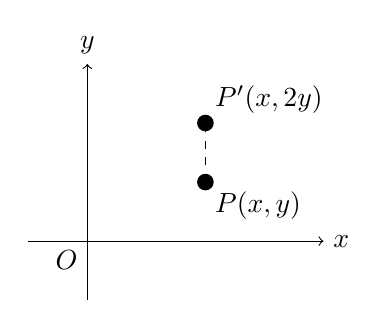
\begin{tikzpicture}[scale=1.5]
    % 绘制坐标轴
    \draw[->] (-0.5,0) -- (2,0) node[right] {$x$};
    \draw[->] (0,-0.5) -- (0,1.5) node[above] {$y$};

    % 绘制原点O
    \coordinate (O) at (0,0);
    \fill (O) circle (0pt) node[anchor=north east] {$O$};
    
    % 绘制旋转前的点P
    \coordinate (P) at (1,0.5);
    \fill (P) circle (2pt) node[anchor=north west] {$P(x, y)$};
    
    % 绘制旋转后的点P'
    \coordinate (P') at (1,1);
    \fill (P') circle (2pt) node[anchor=south west] {$P'(x, 2y)$};
    
    % 绘制连接线和旋转弧
    \draw[dashed] (P) -- (P');
    % \draw[->] (0.5,0.5) -- (0.5,1);
    
\end{tikzpicture}
\caption{伸缩变换示意图\label{fig:伸缩变换}}
\end{figure}

\begin{exercise}

    将直角坐标系 $O x y$ 内每个点的横坐标变为原来的 $k_1$ 倍, 纵坐标变为原来的 $k_2$ 倍 $\left(k_1, k_2\right.$ 均为非零常数) 的伸缩变换, 其坐标变换公式是
    
    \begin{equation}
        \left\{\begin{array}{l}
    x^{\prime}=k_1 x, \\
    y^{\prime}=k_2 y .
    \end{array}\right.
    \label{伸缩变换一般表达式}
    \end{equation}
    
    对应的变换矩阵为 
    
    \begin{equation}
    \left(\begin{array}{cc}k_1 & 0 \\ 0 & k_2\end{array}\right).
    \label{伸缩变换一般矩阵}
    \end{equation}

\end{exercise}

注意到,当$k_1=k_2$时,伸缩变换退化为\textcolor{third}{\bf 平移变换}。


\subsubsection{投影变换}
\label{subsubsec:投影变换}

设 $l$ 是平面内一条给定的直线. 对平面内的任意一点 $P$ 作直线 $l$ 的垂线, 垂足为点 $P^{\prime}$, 则称点 $P^{\prime}$ 为点 $P$ 在直线 $l$ 上的\textcolor{third}{\bf 投影} (projection). 将平面上每一点 $P$ 变成它在直线 $l$ 上的投影 $P^{\prime}$, 这个变换称为关于直线 $l$ 的\textcolor{third}{\bf 投影变换}  .

如图 \ref{fig:投影变换}, 在直角坐标系 $O x y$ 内, 过任意一点 $P$ 作 $x$ 轴的垂线, 垂足为点 $P^{\prime}$, 我们称点 $P^{\prime}$ 为点 $P$ 在 $x$ 轴上的  投影. 如果一个变换把直角坐标系内的每一点变成它在 $x$ 轴上 的投影, 那么称这个变换为关于 $x$ 轴的投影变换.

\begin{figure}[h]
\centering
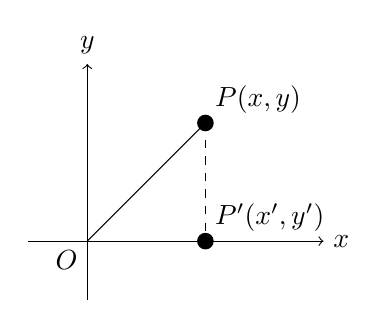
\begin{tikzpicture}[scale=1.5]
    % 绘制坐标轴
    \draw[->] (-0.5,0) -- (2,0) node[right] {$x$};
    \draw[->] (0,-0.5) -- (0,1.5) node[above] {$y$};
    
    % 绘制原点O
    \coordinate (O) at (0,0);
    \fill (O) circle (0pt) node[anchor=north east] {$O$};
    
    % 绘制旋转前的点P
    \coordinate (P) at (1,1);
    \fill (P) circle (2pt) node[anchor=south west] {$P(x, y)$};
    
    % 绘制旋转后的点P'
    \coordinate (P') at (1,0);
    \fill (P') circle (2pt) node[anchor=south west] {$P'(x', y')$};
    
    % 绘制连接线和旋转弧
    \draw[-] (O) -- (P);
    \draw[dashed] (P) -- (P');
    
\end{tikzpicture}
\caption{投影变换示意图\label{fig:投影变换}}
\end{figure}

设在关于 $x$ 轴的投影变换的作用下, 点 $P(x, y)$ 变成 点 $P^{\prime}\left(x^{\prime}, y^{\prime}\right)$。
此时 $x^{\prime}, y^{\prime}$ 与 $x, y$ 有如下关系:

$$
\left\{\begin{array}{l}
x^{\prime}=x, \\
y^{\prime}=0 .
\end{array}\right.
$$

即

$$
\left\{\begin{array}{l}
x^{\prime}= 1 \cdot x + 0 \cdot y, \\
y^{\prime}= 0 \cdot x + 0 \cdot y.
\end{array}\right.
$$

对应的二阶矩阵为 $\left(\begin{array}{ll}1 & 0 \\ 0 & 0\end{array}\right)$.

\subsubsection{切变变换}
\label{subsubsec:切变变换}

\textcolor{third}{\bf 切变变换}(shearing)是一种特殊的几何变换,用于改变物体的形状。它在一个方向上按照一定的比例“拉伸”或“压缩”物体,同时在与这个方向垂直的另一方向上保持物体不变。在二维平面上,切变变换主要有两种:

\begin{itemize}
    \item \textbf{水平切变}:在水平方向上拉伸或压缩物体,与物体在垂直方向上的位置成比例。垂直方向上的形状不会改变。如图\ref{fig:shearing-wiki}\footnote{图源:\url{https://en.wikipedia.org/wiki/Shear\_mapping}}所示。
    \item \textbf{垂直切变}:在垂直方向上拉伸或压缩物体,与物体在水平方向上的位置成比例。水平方向上的形状不会改变。
\end{itemize}


\begin{figure}[!h]
    \centering
    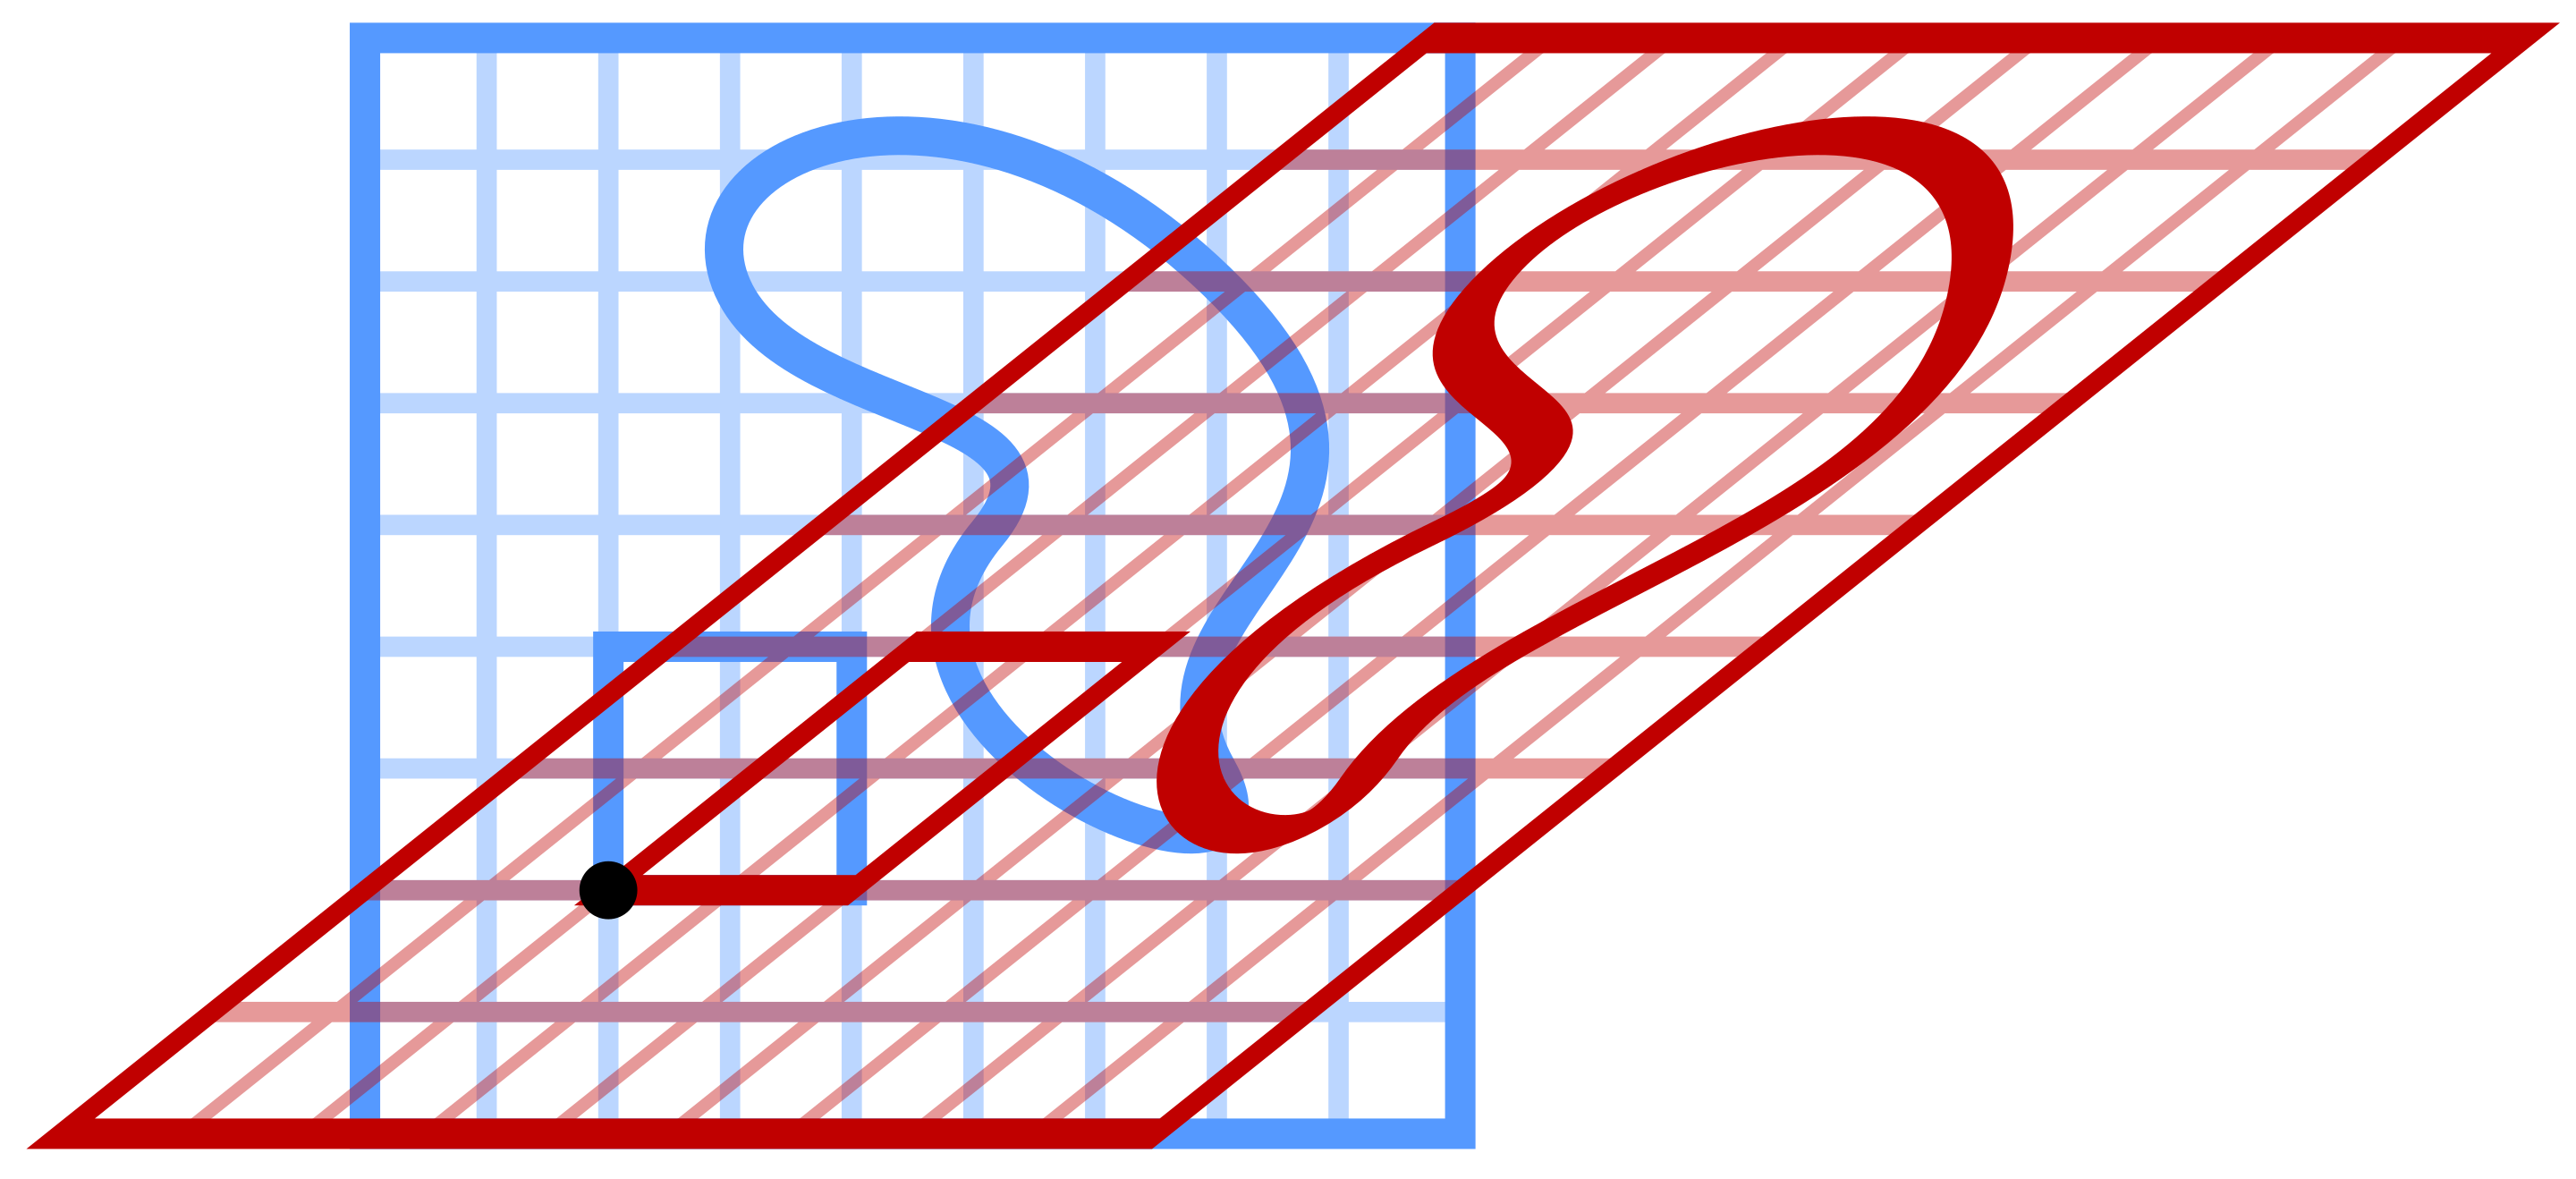
\includegraphics[width=0.4\textwidth]{figure/matrix/shearing.png}
    \caption{平面的水平剪切,将蓝色转变为红色,黑点为原点}
    \label{fig:shearing-wiki}
\end{figure}


如图 \ref{fig:切变变换}, 在直角坐标系 $O x y$ 内, 将每一点 $P(x$, $y$ ) 沿着与 $x$ 轴平行的方向平移 $k y$ 个单位变成点 $P^{\prime}$, 其中 $k$ 是非零常数, 这就是水平切变(或平行于 $x$ 轴的切变变换).
设 $P^{\prime}\left(x^{\prime}, y^{\prime}\right)$, 则
此时 $x^{\prime}, y^{\prime}$ 与 $x, y$ 有如下关系:

$$
\left\{\begin{array}{c}
x^{\prime}=x+k y, \\
y^{\prime}=y .
\end{array}\right.
$$

从而, 对应的二阶矩阵为 $\left(\begin{array}{ll}1 & k \\ 0 & 1\end{array}\right)$.

\begin{figure}[h]
\centering
\begin{tikzpicture}[scale=1.5]
    % 绘制坐标轴
    \draw[->] (-0.5,0) -- (1.5,0) node[right] {$x$};
    \draw[->] (0,-0.5) -- (0,1.5) node[above] {$y$};
    
    % 绘制原点O
    \coordinate (O) at (0,0);
    \fill (O) circle (0pt) node[anchor=north east] {$O$};
    
    % 绘制旋转前的点P
    \coordinate (P) at (0.5,1);
    \fill (P) circle (2pt) node[anchor=south west] {$P(x, y)$};
    
    % 绘制旋转后的点P'
    \coordinate (P') at (1.5,1);
    \fill (P') circle (2pt) node[anchor=south west] {$P'(x+ky, y)$};
    
    % 绘制连接线和旋转弧
    \draw[dashed] (P) -- (P');
    
\end{tikzpicture}
\caption{切变变换示意图\label{fig:切变变换}}
\end{figure}

\begin{exercise}

    平行于 $y$ 轴的切变变换是指将直角坐标系内的每一点 $P(x, y)$ 沿着与 $y$ 轴 平行的方向平移 $k x$ 个单位 (其中 $k$ 是非零常数) 的线性变换. 其坐标变换公式为
    $$
    \left\{\begin{array}{c}
    x^{\prime}=x, \\
    y^{\prime}=k x+y .
    \end{array}\right.
    $$
    对应的矩阵为 $\left(\begin{array}{ll}1 & 0 \\ k & 1\end{array}\right)$.
        
\end{exercise}

\subsection{线性变换及其基本性质}

\begin{proposition}[平面上保持直线性质的变换]
\label{thm:保持直线性质的变换}
设 $T$ 是一个平面到平面的映射($T: \mathbb{R}^2 \rightarrow \mathbb{R}^2$), $\boldsymbol{u}, \boldsymbol{v}$ 是平面上的任意两个向量, $\lambda$ 是一个任意实数。若从原点引出向量$\boldsymbol{u}, \boldsymbol{v}$,其末端点分别记为$P_1,P_2$,显然,只要选取合适的$\boldsymbol{u}, \boldsymbol{v}$,$P_1,P_2$就可以确定出平面上的任意直线。如果 $T$ 满足下面的条件:
\begin{enumerate}
    \item 保加法:$T(\boldsymbol{u}+\boldsymbol{v}) = T(\boldsymbol{u})+T(\boldsymbol{v})$;
    \item 保数乘:$T(\lambda \boldsymbol{u}) =\lambda T(\boldsymbol{u})$.
\end{enumerate}
则该映射不改变直线的形状、平行性、与其他直线的交叉点的位置以及直线上点的相对距离。
\end{proposition}

\begin{proof}

\underline{1. 不改变直线的形状}:直线可以表示为向量的线性组合,即对于两个向量 \(\boldsymbol{u}\) 和 \(\boldsymbol{v}\),直线可以表示为 \(\boldsymbol{u} + t\boldsymbol{v}\),其中 \(t\) 是标量。根据变换$T$的定义,我们有:

\begin{align*}
    T(\boldsymbol{u} + t\boldsymbol{v})
    = & T(\boldsymbol{u}) + T(t\boldsymbol{v})\\
    = & T(\boldsymbol{u}) + tT(\boldsymbol{v})
\end{align*}

即直线在经过这样的变换后仍然是一条直线。

\underline{2. 保持平行性}:考虑两条平行直线,它们可以表示为 \(\boldsymbol{u} + t\boldsymbol{v}\) 和 \(\boldsymbol{u}' + t\boldsymbol{v}\),注意这两条直线共享同一个方向向量 \(\boldsymbol{v}\)。因为变换$T$保持向量加法和标量乘法,变换后的直线分别是 \(T(\boldsymbol{u}) + tT(\boldsymbol{v})\) 和 \(T(\boldsymbol{u}') + tT(\boldsymbol{v})\)。因为它们仍然共享同一个方向向量 \(T(\boldsymbol{v})\),所以变换后的直线保持平行。

\underline{3. 保持交叉点位置}:假设两条直线 \(L_1\) 和 \(L_2\) 在点 \(\boldsymbol{p}\) 交叉,即存在某个 \(t_1\) 和 \(t_2\) 使得 \(\boldsymbol{u} + t_1\boldsymbol{v} = \boldsymbol{u}' + t_2\boldsymbol{v}' = \boldsymbol{p}\)。应用变换 \(T\),我们得到 \(T(\boldsymbol{u} + t_1\boldsymbol{v}) = T(\boldsymbol{u}') + t_2T(\boldsymbol{v}') = T(\boldsymbol{p})\)。这表明变换后的直线在 \(T(\boldsymbol{p})\) 点交叉,保持了交叉点的位置。

\underline{4. 保持直线上点的相对距离}:考虑直线 \(L\) 上的两点 \(\boldsymbol{p}\) 和 \(\boldsymbol{q}\),直线上的任意一点 \(\boldsymbol{x}\) 可以表示为 \(\boldsymbol{p}\) 和 \(\boldsymbol{q}\) 的线性组合:
\[ \boldsymbol{x} = \alpha\boldsymbol{p} + (1-\alpha)\boldsymbol{q} \]
其中,\(\alpha\) 是一个标量。我们将线性变换 \(T\) 应用于直线 \(L\) 上的点 \(\boldsymbol{x}\):
\begin{align*}
    T(\boldsymbol{x}) 
    & = T(\alpha\boldsymbol{p} + (1-\alpha)\boldsymbol{q}) \\
    & = \alpha T(\boldsymbol{p}) + (1-\alpha)T(\boldsymbol{q})    
\end{align*}

这表明,经过线性变换 \(T\) 后,点 \(\boldsymbol{x}\) 依然位于 \(T(\boldsymbol{p})\) 和 \(T(\boldsymbol{q})\) 定义的直线上,并且保持了与原始直线相同的比例 \(\alpha\)。

\end{proof}

到这里,我们证明了平面上保加法和保数乘的变换的向量映射(或称变换)不会改变直线的形状、直线之间的平行和相交关系,也不会改变直线上的点之间的相对距离,我们称这些性质是平面的“线性”性质,而变换$T$可以在变换前后保持这种“线性”性质。

可以验证,在三维空间中,保加法和保数乘的变换仍然可以保持空间的线性性质,具体细节我们就略过了。现在,我们希望对“空间”的概念进行抽象,将研究对象从我们熟悉的二维、三维推广到任意维度。所以我们首先需要给出向量空间的定义。

% \begin{proof}
%     要证明线性变换保持形状、平行性和交叉点的位置,我们可以具体考虑两条直线及其在线性变换下的表现。

% \underline{1. 形状保持}:假设有一条直线 \(L_1\),其方程为 \(y = mx + n\),其中 \(m\) 是斜率,\(n\) 是截距。我们考虑两个点 \(P_1(x_1, y_1),P_2(x_2, y_2)\) 在这条直线上,即 \(y_1 = mx_1 + n, y_2 = mx_2 + n\)。

% 现在,应用变换 \(T\),用矩阵表示为 \(\begin{pmatrix} a & b \\ c & d \end{pmatrix}\),于是有
% \[ T(P_1) = \begin{pmatrix} a & b \\ c & d \end{pmatrix} \begin{pmatrix} x_1 \\ mx_1 + n \end{pmatrix},\quad
% T(P_2) = \begin{pmatrix} a & b \\ c & d \end{pmatrix} \begin{pmatrix} x_2 \\ mx_2 + n \end{pmatrix}
% % = \begin{pmatrix} ax + b(mx + n) \\ cx + d(mx + n) \end{pmatrix} 
% % = \begin{pmatrix} (a + bm) x + bn \\ (c + dm)x + dn \end{pmatrix} 
% \]
% 可以验证,变换后的点 \(T(P_1), T(P_2)\) 处在一条斜率为$\frac{bm}{a}$的直线上,这表明原来直线的“形状”(即“直的线”)得到了保持\textcolor{red}{(验证过程留做习题)}。

% \underline{2. 平行性保持}:考虑两条平行直线 \(L_1: y = m_1x + n_1\) 和 \(L_2: y = m_2x + n_2\),因为它们平行,所以 \(m_1 = m_2\)。

% 应用变换 \(T\) 到这两条直线上,我们可以得到新的两条直线。计算出两条新直线的斜率可以发现二者仍然相等,即保持了平行性\textcolor{red}{(验证过程留做习题)}。

% \underline{3. 交叉点保持}:假设两条直线 \(L_1: y = m_1x + n_1\) 和 \(L_2: y = m_2x + n_2\) 交于点 \(P(x, y)\),即满足
% \[ m_1x + n_1 = m_2x + n_2 \]
% 解这个方程可以得到交点 \(P\) 的坐标。在变换 \(T\) 下,两条直线变为 \(T(L_1)\) 和 \(T(L_2)\)。
% 可以验证,\(T(L_1)\) 和 \(T(L_2)\)的交点为$T(P)$\textcolor{red}{(验证过程留做习题)}。
% % 由于线性变换是结构保持的,原有的交点 \(P\) 在变换后的直线上的对应点 \(T(P)\) 保持为这两条新直线的交点。换句话说,如果两条直线在变换前相交,它们在变换后仍然相交于对应的点,这是因为线性变换保持了方程组的解的结构,即交点。

% \end{proof}

% 证明的关键点:

% \begin{itemize}
%     \item 形状保持的证明关键在于展示变换\(T\)的作用下,直线方程仍保持为直线方程,即证明变换后的输出仍满足直线方程的一般形式。
%     \item 平行性保持的证明依赖于展示如果两直线在变换前平行(斜率相等),则在变换后仍然平行。这可以通过比较变换后两条直线的斜率来证明。
%     \item 交叉点保持的证明需要表明如果两直线在变换前有交点,那么在变换后它们仍然会在某点交汇,且该点是原交点变换后的点。
% \end{itemize}

\begin{definition}[线性变换]
    \textcolor{third}{\bf 线性变换}是从一个向量空间到另一个向量空间的函数 \(f: V \rightarrow W\),对于所有的 \(x, y \in V\) 和任意标量 \(a, b\),满足以下两个条件:

    \begin{enumerate}
        \item \textbf{加法保持性:}\(f(x + y) = f(x) + f(y)\)
        \item \textbf{数量乘法保持性:}\(f(ax) = af(x)\)
    \end{enumerate}
\end{definition}

\begin{note}
  让学生回顾之前展示的每个变换,并提醒他们每个变换都保持了直线的性质。
\end{note}

\vspace*{0.5cm}

为了研究线性变换的性质, 我们先定义平面向量的加法和数量乘法。

\begin{definition}[平面向量的加法]
  设向量 $\boldsymbol{u}=\left(\begin{array}{l}x_1 \\ y_1\end{array}\right), \boldsymbol{v}=\left(\begin{array}{l}x_2 \\ y_2\end{array}\right)$, 
  规定向量 $\boldsymbol{u}$ 与 $\boldsymbol{v}$ 的和 $\boldsymbol{u}+\boldsymbol{v}=\left(\begin{array}{l}x_1+x_2 \\ y_1+y_2\end{array}\right)$.
\end{definition}

\begin{note}
向量加法就是高中学的平行四边形法则。
\end{note}

\begin{definition}[平面向量的数量乘法]
  设向量 $\boldsymbol{u}=\left(\begin{array}{l}x \\ y\end{array}\right)$, 
  规定实数 $\lambda$ 与向量 $\boldsymbol{u}$ 的乘积 $\lambda \boldsymbol{u}=\left(\begin{array}{l}\lambda x \\ \lambda y\end{array}\right)$; 
\end{definition}

平面向量的数量乘法之所以被称为"数量乘法"是因为它涉及到一个向量与一个数(或者我们可以称之为标量)相乘的操作。这个数可以是任何实数。当我们将一个向量与一个数相乘时,结果是一个新的向量,它的方向与原始向量相同(或相反),但长度(或称为模)被缩小或拉大了。这个操作影响到向量的大小,所以我们称之为"数量乘法"。


\begin{exercise}

  \begin{enumerate}
    \item   【高中数学人教A版选修4-2】设向量 $\boldsymbol{u}=\left(\begin{array}{l}1 \\ 2\end{array}\right), \boldsymbol{v}=\left(\begin{array}{l}2 \\ 1\end{array}\right)$. 
            如图 \ref{fig:vector-addition-reflection}, 先利用平行四边形法则求 $\boldsymbol{u}+\boldsymbol{v}$, 再对向量 $(\boldsymbol{u}+\boldsymbol{v})$ 进行关于 $x$ 轴的反射变换; 
            或者, 先对向量 $\boldsymbol{u}, \boldsymbol{v}$ 做关于 $x$ 轴的反射变换, 
            再利用平行四边形法则求反射变换后的两个向量的和.请回答下列问题:

            \begin{enumerate}
              \item 这两个过程的结果相同吗?
              \item 如果把$\boldsymbol{u}$关于$x$轴的反射变换记作$\text{Reflect}_{x}(\boldsymbol{u})$,
              把$\boldsymbol{v}$关于$x$轴的反射变换记作$\text{Reflect}_{x}(\boldsymbol{v})$,
              把$\boldsymbol{u}+\boldsymbol{v}$关于$x$轴的反射变换记作$\text{Reflect}_{x}(\boldsymbol{u}+\boldsymbol{v})$,
              那么,这些变换的坐标变换矩阵分别是什么?这些变换的矩阵有什么关系?
            \end{enumerate}

            \begin{figure}[!h]
            \centering
            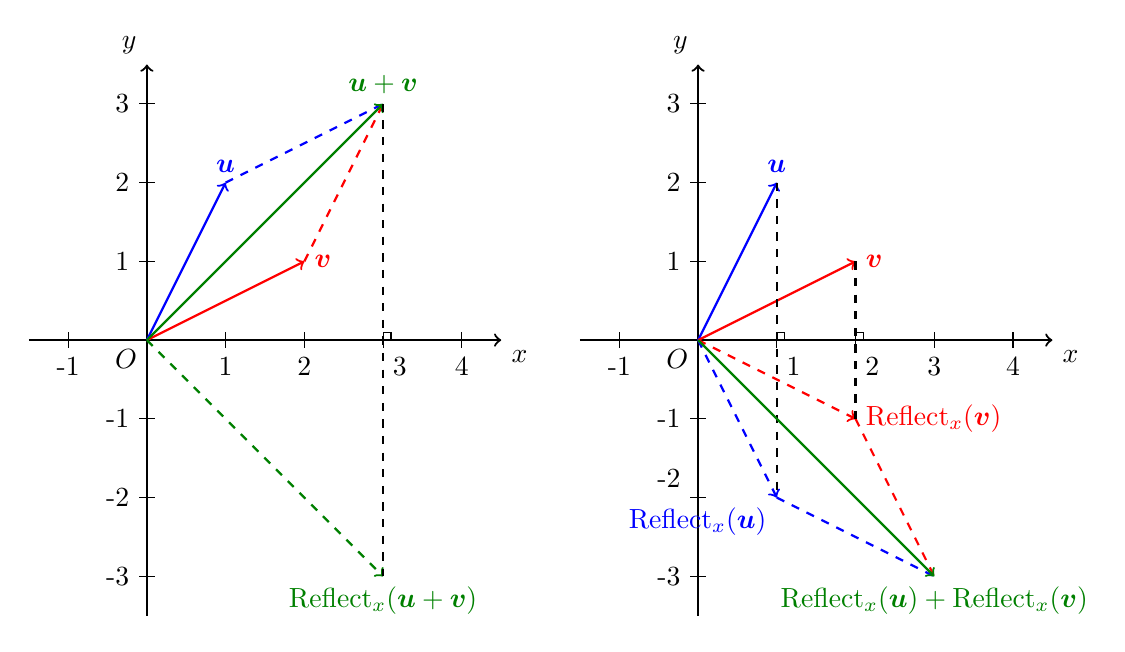
\begin{tikzpicture}[scale=1, transform shape]

              % First diagram: Vector addition first, then reflection
              \begin{scope}[shift={(0,0)}]

                \foreach \x in {-1,0,...,4} {
                  \ifnum \x = 0
                  \else
                        \ifnum \x = 3
                            \draw (\x, 0.1) -- (\x, -0.1) node[below right] {\x};
                        \else
                            \draw (\x, 0.1) -- (\x, -0.1) node[below] {\x};
                        \fi
                  \fi
                }

                \foreach \y in {-3,-2,...,3} {
                    \ifnum \y = 0
                    \else
                        \draw (0.1, \y) -- (-0.1, \y) node[left] {\y};
                    \fi
                }

                % Draw origin
                \node at (0,0) [below left] {$O$};

                % Draw axes
                \draw[thick,->] (-1.5,0) -- (4.5,0) node[anchor=north west] {$x$};
                \draw[thick,->] (0,-3.5) -- (0,3.5) node[anchor=south east] {$y$};
              
                % Draw original vectors alpha and beta
                \draw[thick,->,blue] (0,0) -- (1,2) node[anchor=south] {$\boldsymbol{u}$};
                \draw[thick,->,red] (0,0) -- (2,1) node[anchor=west] {$\boldsymbol{v}$};

                \draw[thick,-,blue,dashed] (1,2) -- (3,3);
                \draw[thick,-,red,dashed] (2,1) -- (3,3);
              
                % Draw alpha + beta
                \draw[thick,->,mygreen] (0,0) -- (3,3) node[anchor=south] {$\boldsymbol{u}+\boldsymbol{v}$};
              
                % Draw reflection of alpha + beta
                \draw[thick,->,mygreen,dashed] (0,0) -- (3,-3) node[anchor=north] {$\text{Reflect}_{x}(\boldsymbol{u}+\boldsymbol{v})$};

                \draw[thick,-,black,dashed] (3,3) -- (3,-3);

                % Add a right-angle symbol (perpendicular mark)
                \draw (3,0) -- (3,0.1) -- (3+0.1,0.1) -- (3+0.1,0);

              \end{scope}
              
              % Second diagram: Reflection first, then vector addition
              \begin{scope}[shift={(7,0)}]

                \foreach \x in {-1,0,...,4} {
                  \ifnum \x = 0
                    % Do nothing when \x is 0
                  \else
                    \ifnum \x = 1
                      \draw (\x, 0.1) -- (\x, -0.1) node[below right] {\x};
                    \else
                      \ifnum \x = 2
                        \draw (\x, 0.1) -- (\x, -0.1) node[below right] {\x};
                      \else
                        \draw (\x, 0.1) -- (\x, -0.1) node[below] {\x};
                      \fi
                    \fi
                  \fi
                }                

                \foreach \y in {-3,-2,...,3} {
                    \ifnum \y = 0
                    \else
                        \ifnum \y = -2
                            \draw (0.1, \y) -- (-0.1, \y) node[above left] {\y};
                        \else
                            \draw (0.1, \y) -- (-0.1, \y) node[left] {\y};
                        \fi
                    \fi
                  }

                % Draw origin
                \node at (0,0) [below left] {$O$};

                % Draw axes
                \draw[thick,->] (-1.5,0) -- (4.5,0) node[anchor=north west] {$x$};
                \draw[thick,->] (0,-3.5) -- (0,3.5) node[anchor=south east] {$y$};

                % Draw original vectors alpha and beta
                \draw[thick,->,blue] (0,0) -- (1,2) node[anchor=south] {$\boldsymbol{u}$};
                \draw[thick,->,red] (0,0) -- (2,1) node[anchor=west] {$\boldsymbol{v}$};
              
                % Draw reflection of alpha and beta
                \draw[thick,->,blue,dashed] (0,0) -- (1,-2) node[anchor=north east] {$\text{Reflect}_{x}(\boldsymbol{u})$};
                \draw[thick,->,red,dashed] (0,0) -- (2,-1) node[anchor=west] {$\text{Reflect}_{x}(\boldsymbol{v})$};

                \draw[thick,-,blue,dashed] (1,-2) -- (3,-3);
                \draw[thick,-,red,dashed] (2,-1) -- (3,-3);

                \draw[thick,-,black,dashed] (1,2) -- (1,-2);
                \draw[thick,-,black,dashed] (2,1) -- (2,-1);
                
                % Add a right-angle symbol (perpendicular mark)
                \draw (1,0) -- (1,0.1) -- (1+0.1,0.1) -- (1+0.1,0);
                \draw (2,0) -- (2,0.1) -- (2+0.1,0.1) -- (2+0.1,0);

                % Draw addition of reflected alpha and beta
                \draw[thick,->,mygreen] (0,0) -- (3,-3) node[anchor=north] {$\text{Reflect}_{x}(\boldsymbol{u}) + \text{Reflect}_{x}(\boldsymbol{v})$};

              \end{scope}

            \end{tikzpicture}
            \caption{向量加法与反射变换}
            \label{fig:vector-addition-reflection}
            \end{figure}

  \item 设向量 $\boldsymbol{u}=\left(\begin{array}{l}2 \\ 1\end{array}\right)$ ,
        如图 \ref{fig:vector-scaling}, 先用$2$与该向量进行数量乘法,再使向量在 \( x \)-轴方向的坐标变为原来的 3 倍,同时使 \( y \)-轴方向的坐标变为原来的 2 倍;
        或者,先使向量在 \( x \)-轴方向的坐标变为原来的 3 倍,同时使 \( y \)-轴方向的坐标变为原来的 2 倍,再用$2$与该向量进行数量乘法。
        请回答下列问题:

        \begin{enumerate}
          \item 这两个过程的结果相同吗?
          \item 如果把$\boldsymbol{u}$的伸缩变换记作$\text{Stretch}(\boldsymbol{u})$,
          把$2\boldsymbol{u}$的伸缩变换记作$\text{Stretch}(2\boldsymbol{u})$,
          那么,这些变换的坐标变换矩阵分别是什么?这些变换的矩阵有什么关系?
        \end{enumerate}

        \begin{figure}[!h]
          \centering
          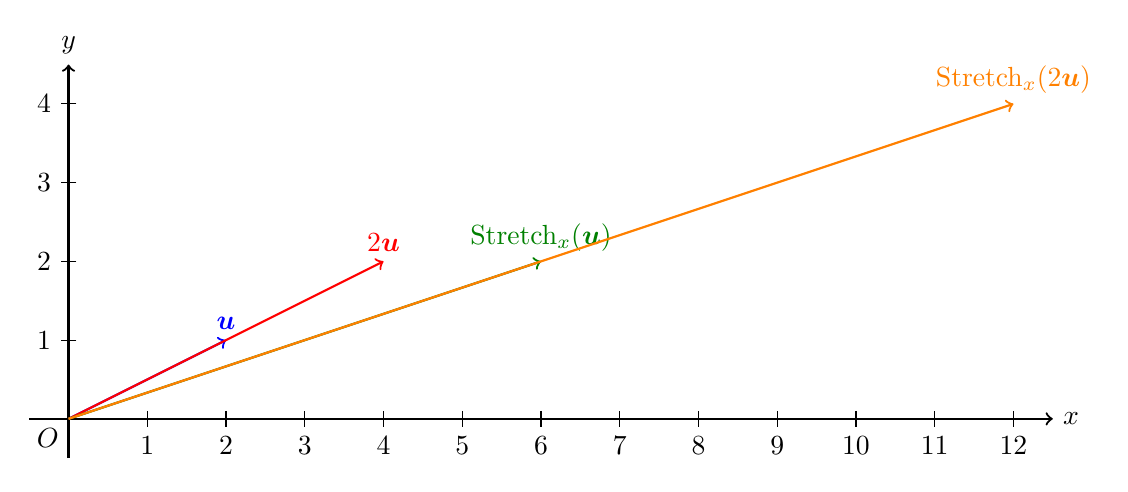
\begin{tikzpicture}[scale=1, transform shape]

            \foreach \x in {1,2,...,12} {
                \draw (\x, 0.1) -- (\x, -0.1) node[below] {\x};
            }

            \foreach \y in {1,2,...,4} {
                \draw (0.1, \y) -- (-0.1, \y) node[left] {\y};
            }

            % 绘制原点O
            \node at (0,0) [below left] {$O$};

            % Draw axes
            \draw[thick,->] (-0.5,0) -- (12.5,0) node[right] {$x$};
            \draw[thick,->] (0,-0.5) -- (0,4.5) node[above] {$y$};
          
            % Original vector v
            \draw[thick,->,blue] (0,0) -- (2,1) node[above] {$\boldsymbol{u}$};
            
            % Scaled vector 2v
            \draw[thick,->,red] (0,0) -- (4,2) node[above] {$2\boldsymbol{u}$};
          
            % Transformed vector T(v)
            \draw[thick,->,mygreen] (0,0) -- (6,2) node[above] {$\text{Stretch}_{x}(\boldsymbol{u})$};
          
            % Transformed vector T(2v)
            \draw[thick,->,orange] (0,0) -- (12,4) node[above] {$\text{Stretch}_{x}(2\boldsymbol{u})$};
          
          \end{tikzpicture}
          \caption{向量伸缩变换}
          \label{fig:vector-scaling}
        \end{figure}

  \end{enumerate}

\end{exercise}

\begin{theorem}[线性变换的性质]
\label{thm:线性变换的性质}
设 $T$ 是平面上一个线性变换, $\boldsymbol{u}, \boldsymbol{v}$ 是平面上的任意两个向量, $\lambda$ 是一个任意实数, 则
\begin{enumerate}
  \item $T(u+v) =T(u)+T(v)$;
  \item $T(\lambda u) =\lambda T(u)$.
\end{enumerate}

\end{theorem}

综合上述两条性质, 可以得到:

设 $T$ 是平面上一个线性变换, $\boldsymbol{u}, \boldsymbol{v}$ 是平面上的任意两个向量, $\lambda_1, \lambda_2$ 是任意两个 实数, 则
\begin{equation}
  T\left(\lambda_1 \boldsymbol{u}+\lambda_2 \boldsymbol{v}\right)=\lambda_1 T (\boldsymbol{u})+\lambda_2 T (\boldsymbol{v})
\end{equation}

\begin{note}
  在很多数学教材中使用定理\ref{thm:线性变换的性质}中的两条性质作为线性变换的定义。
  可以验证,任何满足这两条性质的变换都能够保持直线的性质,即不改变直线的形状、平行性和交叉点的位置。
\end{note}

\section{矩阵的运算}

\subsection{向量与向量间的乘法运算}

在介绍矩阵的运算之前我们首先回顾向量之间的乘法运算。存在两种类型的向量与向量的乘积:内积和外积。

\begin{definition}[内积] \label{def:inner-product} 
对 $x, y \in \mathbb{R}^n$, 我们有:
$$
x^T y=\sum_{i=1}^n x_i y_i \in \mathbb{R}
$$
\end{definition}

\begin{exercise}\label{exer:01}
假设我们有两个二维向量 $x = \begin{bmatrix} 1 \\ 2 \end{bmatrix}$ 和 $y = \begin{bmatrix} 3 \\ 4 \end{bmatrix}$。我们可以使用定义 \ref{def:inner-product} 中的公式来计算它们的内积:

\[
x^T y = x y^T = \begin{bmatrix} 1 & 2 \end{bmatrix} \begin{bmatrix} 3 \\ 4 \end{bmatrix} = (1 \cdot 3) + (2 \cdot 4) = 3 + 8 = 11
\]

因此,向量 $x$ 和 $y$ 的内积为 $11$。
\end{exercise}

\begin{definition}[外积] \label{def:outer-product} 
对 $x \in \mathbb{R}^m, y \in \mathbb{R}^n$, 我们有:
$$
x y^T=\left(\begin{array}{ccc}
x_1 y_1 & \cdots & x_1 y_n \\
\vdots & & \vdots \\
x_m y_1 & \cdots & x_m y_n
\end{array}\right) \in \mathbb{R}^{m \times n}
$$
\end{definition}

\begin{exercise}
    假设我们有一个列向量 $x = \begin{bmatrix} 1 \\ 2 \end{bmatrix}$ 和一个三维向量 $y = \begin{bmatrix} 3 \\ 4 \\ 5 \end{bmatrix}$。我们可以使用定义 \ref{def:outer-product} 中的公式来计算它们的外积:

\[
x y^T = \begin{bmatrix} 1 \\ 2 \end{bmatrix} \begin{bmatrix} 3 & 4 & 5 \end{bmatrix}
\]

计算这个外积:

\[
x y^T = \begin{bmatrix}
1 \cdot 3 & 1 \cdot 4 & 1 \cdot 5 \\
2 \cdot 3 & 2 \cdot 4 & 2 \cdot 5 \\
\end{bmatrix} = \begin{bmatrix}
3 & 4 & 5 \\
6 & 8 & 10 \\
\end{bmatrix}
\]

因此,列向量 $x$ 和三维向量 $y$ 的外积是一个 $2 \times 3$ 的矩阵。
\end{exercise}


\subsection{用矩阵做线性变换}

在第\ref{subsec:几种特殊几何变换}节中,我们通过将线性变换写成坐标变换方程的方法,
指出平面上线性变换和二阶方阵之间存在着一一对应的关系,即我们实现了用矩阵表示线性变换。

此外,我们之前提到,矩阵源于人们在解方程组是对简洁表达的需求。
那么,不借助坐标变换方程,我们可否直接用矩阵来实现坐标变换呢?答案是肯定的.

让我们回顾一下式(\ref{eq:旋转变换的坐标变换公式}),在直角坐标系 $O x y$ 内, 
将任意一点$P(x, y)$绕原点 $O$ 按逆时针方向旋转 $\theta$ 角得到点$P^{\prime}(x^{\prime}, y^{\prime})$的旋转变换的坐标变换公式

\begin{equation*}
  \left\{\begin{array}{l}
  x^{\prime}=x \cos \theta-y \sin \theta, \\
  y^{\prime}=x \sin \theta+y \cos \theta .
  \end{array}\right.    
\end{equation*}

我们进行如下规定,就可以实现用矩阵来做坐标变换

% Define custom colors
\definecolor{softgreen}{rgb}{0.7, 1.0, 0.7}
\definecolor{softblue}{rgb}{0.7, 0.7, 1.0}
\definecolor{coralred}{rgb}{1.0, 0.5, 0.5}
\definecolor{softorange}{rgb}{1.0, 0.8, 0.6}
\definecolor{softyellow}{rgb}{1.0, 1.0, 0.7}

% % Define custom column types with background colors
% \newcolumntype{S}{>{\columncolor{softgreen}}c}
% \newcolumntype{R}{>{\columncolor{coralred}}c}

\begin{equation*}
  \left(\begin{array}{c}
    \cellcolor{softyellow} x^{\prime} \\
    \cellcolor{softorange} y^{\prime}
  \end{array}\right)=\left(\begin{array}{cc}
    \cellcolor{softgreen} \cos \theta & \cellcolor{softgreen} -\sin \theta \\
    \cellcolor{softblue} \sin \theta & \cellcolor{softblue} \cos \theta
    \end{array}\right) \cdot \left(\begin{array}{>{\columncolor{coralred}}c}
  x \\
  y
  \end{array}\right)=\left(\begin{array}{c}
    \cellcolor{softyellow} (\cos \theta) \cdot x + (-\sin \theta) \cdot y \\
    \cellcolor{softorange} (\sin \theta) \cdot x + (\cos \theta) \cdot y
    \end{array}\right)
\end{equation*}

我们把第一个等号对应的关系称为\textcolor{third}{\bf 矩阵与向量间的乘法运算}。
将一个矩阵与一个向量相乘,就是对该向量进行该矩阵所表示的线性变换。

\begin{note}
  学生可以尝试把之前的几何变换的坐标变换公式写成矩阵与向量间的乘法运算。
\end{note}

\subsection{矩阵与向量间的乘法运算}

\begin{definition}[矩阵与向量间的乘法运算] \label{def:mat-vec-multi}

矩阵 $A \in \mathbb{R}^{m \times n}$ 和向量 $x \in \mathbb{R}^n$ 的乘积是一个大小为 $\mathbb{R}^m$ 的向量, 满足:

$$
A x=\left(\begin{array}{c}
a_{r, 1}^T x \\
\vdots \\
a_{r, m}^T x
\end{array}\right)=\sum_{i=1}^n a_{c, i} x_i \in \mathbb{R}^m
$$

其中 $a_{r, i}^T$ 是行向量, $a_{c, j}$ 是 $A$ 的列向量, $x_i$ 是 $x$ 的元素。
\end{definition}

\begin{exercise}
    假设我们有一个2x3的矩阵 $A$ 与一个3维向量 $x$ 相乘。

矩阵 $A$ 和向量 $x$ 的值如下:

\[
A = \begin{bmatrix}
1 & 2 & 3 \\
4 & 5 & 6 \\
\end{bmatrix}
\]

\[
x = \begin{bmatrix}
2 \\
3 \\
1 \\
\end{bmatrix}
\]

现在,让我们根据定义,计算 $Ax$ 的乘积:

\[
Ax = \begin{bmatrix}
1 & 2 & 3 \\
4 & 5 & 6 \\
\end{bmatrix} \begin{bmatrix}
2 \\
3 \\
1 \\
\end{bmatrix}
\]

我们首先计算每一行与向量 $x$ 的内积,然后将结果组合成一个新的向量:

1. 第一行与 $x$ 的内积: $a_{1,1}^T x = \begin{bmatrix} 1 & 2 & 3 \end{bmatrix} \begin{bmatrix} 2 \\ 3 \\ 1 \end{bmatrix} = 1 \cdot 2 + 2 \cdot 3 + 3 \cdot 1 = 2 + 6 + 3 = 11$

2. 第二行与 $x$ 的内积: $a_{2,1}^T x = \begin{bmatrix} 4 & 5 & 6 \end{bmatrix} \begin{bmatrix} 2 \\ 3 \\ 1 \end{bmatrix} = 4 \cdot 2 + 5 \cdot 3 + 6 \cdot 1 = 8 + 15 + 6 = 29$

因此,$Ax$ 的结果是一个大小为 $\mathbb{R}^2$ 的向量,其元素分别是 $11$ 和 $29$。
\end{exercise}

\subsection{初等变换与矩阵的乘法}

\begin{proposition}[TODO]
    特别重要,\textcolor{red}{任意矩阵左乘初等矩阵就相当于做初等行变换,右乘初等矩阵就相当于做初等列变换。}那么如果说任何矩阵都可以通过初等行变换化为上三角,通过初等列变化化为下三角,那么就可以把任意矩阵分解成对角矩阵和一堆初等矩阵的乘积,比如$A=P_{1}^{T}P_{2}^{T}\cdots P_{s}^{T}\Lambda Q_{1} Q_{2} \cdots Q_{t}$
\end{proposition}

\begin{note}
这一节主要是要让学生明白向量/矩阵的乘法核心是\textcolor{red}{“行乘列”}。
\end{note}

\subsection{矩阵与矩阵间的乘法运算}

\begin{definition}[矩阵和矩阵的乘法] \label{def:mat-mat-multi}
    
矩阵 $A \in \mathbb{R}^{m \times n}$ 和 $B \in \mathbb{R}^{n \times p}$ 的乘积是一个大小为 $\mathbb{R}^{n \times p}$ 的矩阵, 满足:

$$
A B=\left(\begin{array}{ccc}
a_{r, 1}^T b_{c, 1} & \cdots & a_{r, 1}^T b_{c, p} \\
\vdots & & \vdots \\
a_{r, m}^T b_{c, 1} & \cdots & a_{r, m}^T b_{c, p}
\end{array}\right)=\sum_{i=1}^n a_{c, i} b_{r, i}^T \in \mathbb{R}^{n \times p}
$$

其中 $a_{r, i}^T, b_{r, i}^T$ 是行向量, $a_{c, j}, b_{c, j}$ 分别是 $A$ 和 $B$ 的列向量。
\end{definition}

\begin{exercise}
    我们将使用一个2x3的矩阵 $A$ 与一个3x2的矩阵 $B$ 相乘。

首先,让我们定义矩阵 $A$ 和矩阵 $B$:

\[
A = \begin{bmatrix}
1 & 2 & 3 \\
4 & 5 & 6 \\
\end{bmatrix}
\]

\[
B = \begin{bmatrix}
2 & 3 \\
4 & 5 \\
6 & 7 \\
\end{bmatrix}
\]

现在,让我们使用这个新的矩阵 $B$ 与之前定义的矩阵 $A$ 相乘,以演示矩阵乘法的过程:

\[
AB = \begin{bmatrix}
1 & 2 & 3 \\
4 & 5 & 6 \\
\end{bmatrix} \begin{bmatrix}
2 & 3 \\
4 & 5 \\
6 & 7 \\
\end{bmatrix}
\]

计算每一行与每一列的内积,并生成新的矩阵 $AB$:

1. 第一行与第一列的内积: $a_{1,1}^T b_{1,1} = \begin{bmatrix} 1 & 2 & 3 \end{bmatrix} \begin{bmatrix} 2 \\ 4 \\ 6 \end{bmatrix} = 1 \cdot 2 + 2 \cdot 4 + 3 \cdot 6 = 2 + 8 + 18 = 28$

2. 第一行与第二列的内积: $a_{1,1}^T b_{2,1} = \begin{bmatrix} 1 & 2 & 3 \end{bmatrix} \begin{bmatrix} 3 \\ 5 \\ 7 \end{bmatrix} = 1 \cdot 3 + 2 \cdot 5 + 3 \cdot 7 = 3 + 10 + 21 = 34$

3. 第二行与第一列的内积: $a_{2,1}^T b_{1,1} = \begin{bmatrix} 4 & 5 & 6 \end{bmatrix} \begin{bmatrix} 2 \\ 4 \\ 6 \end{bmatrix} = 4 \cdot 2 + 5 \cdot 4 + 6 \cdot 6 = 8 + 20 + 36 = 64$

4. 第二行与第二列的内积: $a_{2,1}^T b_{2,1} = \begin{bmatrix} 4 & 5 & 6 \end{bmatrix} \begin{bmatrix} 3 \\ 5 \\ 7 \end{bmatrix} = 4 \cdot 3 + 5 \cdot 5 + 6 \cdot 7 = 12 + 25 + 42 = 79$

因此,$AB$ 的结果是一个大小为 $\mathbb{R}^{2 \times 2}$ 的矩阵,其元素如下:

\[
AB = \begin{bmatrix}
28 & 34 \\
64 & 79 \\
\end{bmatrix}
\]

\end{exercise}

\textcolor{red}{\bf 讲到这里记得回去解释单位矩阵的定义。}


%%%%%%%%%%%%%%%%%%%%%%%%%%%%%%%%%%%%%%%%%%%
\section{基础矩阵操作}

\begin{proposition}[TODO]

\begin{itemize}
    \item  矩阵转置的性质$(AB)^{T}=B^{T} A^{T}$
    \item 逆矩阵的本质是线性变换的逆变换,举例说明,并求给出用单位阵辅助求出逆矩阵的方法,介绍转置的性质$(AB)^{-1}=B^{-1} A^{-1}$最后给出python做法;
    \item 矩阵的行列式的计算方法(只讲二阶和三阶),并讲清楚几何意义:面积比和右手螺旋定则;
    \item 介绍矩阵的迹,以及特殊矩阵的行列式和他们的迹的关系。
\end{itemize}

\end{proposition}

\subsection{矩阵的转置}

\begin{definition}
    
矩阵 $A \in \mathbb{R}^{m \times n}$ 的转置, 记作 $A^T$, 是其中元素的翻转
$$
\forall i, j, \quad A_{i, j}^T=A_{j, i}
$$
\end{definition}

\begin{exercise}
    假设我们有一个 $2 \times 3$ 的矩阵:

$$
A = \begin{bmatrix}
1 & 2 & 3 \\
4 & 5 & 6 \\
\end{bmatrix}
$$

现在,让我们计算矩阵 $A$ 的转置 $A^T$。转置操作将原矩阵的行变成列,列变成行,如下所示:

$$
A^T = \begin{bmatrix}
1 & 4 \\
2 & 5 \\
3 & 6 \\
\end{bmatrix}
$$

这里,我们可以清晰地看到原始矩阵 $A$ 的行变成了 $A^T$ 的列,而原始矩阵的列变成了 $A^T$ 的行。

\end{exercise}

\begin{theorem}[转置运算的性质] \label{thm:transpose-property}
    对矩阵 $A, B$, 我们有 $(A B)^T=B^T A^T$。\textcolor{red}{(提示:想一下矩阵相乘的尺寸对齐关系)}
\end{theorem}

\subsection{矩阵的逆}

\begin{definition} \label{def:invertible-mat}
    给定一个 $n$ 阶方阵 $\mathbf{A}$, 若存在一个 $n$ 阶方阵 $\mathbf{B}$, 使得 $\mathbf{A B}=\mathbf{B} \mathbf{A}=\mathbf{I}_n$, 其中 $\mathbf{I}_n$ 为 $n$ 阶单位矩阵, 则称 $\mathbf{A}$ 是可逆的, 且 $\mathbf{B}$ 是 $\mathbf{A}$ 的逆矩 阵, 记作 $\mathbf{A}^{-1}$ 。
\end{definition}

根据定义\ref{def:invertible-mat},有
$$
A A^{-1}=A^{-1} A=I
$$

不是所有方阵都是可逆的。不可逆矩阵也叫奇异矩阵或退化矩阵,它们的特点是行列式的值为0。下面是一些不可逆矩阵的例子:

\begin{enumerate}
\item 全零矩阵:
   \[
   \begin{bmatrix}
   0 & 0 \\
   0 & 0 \\
   \end{bmatrix}
   \]

\item 含有线性相关行或列的矩阵:
   \[
   \begin{bmatrix}
   1 & 2 \\
   2 & 4 \\
   \end{bmatrix}
   \]

\item 非方矩阵也是不可逆的,例如:
   \[
   \begin{bmatrix}
   1 & 2 \\
   \end{bmatrix}
   \]

\item 任何行或列全为0的矩阵,例如:
   \[
   \begin{bmatrix}
   1 & 0 \\
   0 & 0 \\
   \end{bmatrix}
   \]
\end{enumerate}

这些例子中的矩阵都不能找到一个逆矩阵来满足矩阵乘法的单位矩阵条件。

\begin{theorem}[矩阵的逆运算的性质]
    对可逆矩阵 $A, B$, 我们有 $(A B)^{-1}=B^{-1} A^{-1}$。\textcolor{red}{(提示:套定义和原矩阵相乘就可以证明)}
\end{theorem}

使用Python求矩阵的逆:

\lstinputlisting[language=Python]{scripts/code-unnamed-用python求解矩阵的逆.py}


%%%%%%%%%%%%%%%%%%%%%%%%%%%%%%%%%%%%%
\chapter{函数与优化}

在数学中,\textcolor{main}{\bf 函数}是一个基本但强大的工具,它简单地将每一个输入值映射到一个输出值。你可以将它想象为一个机器:你放进一个数(输入),它便会给你另一个数(输出)。

接下来我们将探讨\textcolor{main}{\bf 优化}的概念,它涉及到一个目标函数的最大化或最小化过程,帮助我们在可能的解决方案中找到“最优”的一种。在现实生活中,这可以是找到最省钱的购物清单,或是找到最快的到达目的地的路线。

在本章中,我们将初步探讨函数和优化的基本理论,为你打开一扇理解和掌握这两个强大工具的大门,从而在实际应用中找到最佳的解决方案。

\section{函数的概念和性质}
\subsection{函数的定义}

\begin{note}
    函数是一种数学关系,它将一个集合的元素映射到另一个集合的元素。
\end{note}

\begin{definition}[函数]
给定两个\textcolor{red}{实数集} $D$ 和 $M$, 若有\textcolor{red}{对应法则} $f$, 使对 $D$ 内每一个数 $x$,都有\textcolor{red}{唯一}的一个数 $y \in M$ 与它相对应,则称 $f$ 是定义在数集 $D$上的\textcolor{third}{\bf 函数},记作
\begin{equation}
\begin{aligned}
    f:D & \rightarrow M, \\
    x & \mapsto y.
\end{aligned}
\end{equation}

数集$D$称为函数$f$的\textcolor{third}{\bf 定义域},$x$所对应的数$y$称为$f$在点$x$的\textcolor{third}{\bf 函数值},常记为$f(x)$.全体函数值的集合

\begin{equation*}
    f(D) = \{y\mid y=f(x),x\in D\} (\subset M)
\end{equation*}

称为函数$f$的\textcolor{third}{\bf 值域}.

\end{definition}

% 其中,$f(x)$ 表示函数 $f$ 对于\textcolor{third}{\bf 输入} $x$ 的\textcolor{third}{\bf 输出};$D(f)$ 表示函数的\textcolor{third}{\bf 定义域}(domain),即函数可以接受的输入值的集合;$R(f)$ 表示函数的\textcolor{third}{\bf 值域}(range),即函数实际输出的值的集合。


%TODO%
关于函数的定义,我们做如下几点说明:

\begin{enumerate}
    \item 什么是函数相同?相同的函数形式可能不同;
    \item 使运算式子有意义的自变量值的全体,称为存在域。函数的定义域常取存在域;
    \item 函数是一种映射关系,原象和象是映射关系的要素;
    \item 在函数定义中, 对每一个 $x \in D$, 只能有唯一的一个 $y$ 值与它对应, 这样 定义的函数称为\textcolor{third}{\bf 单值函数}. 若同一个 $x$ 值可以对应多于一个的 $y$ 值, 则称这种函数为\textcolor{third}{\bf 多值函数}. 在本讲义范围内, 我们只讨论单值函数.
\end{enumerate}

\subsection{具有某些特性的函数}

\subsubsection{有界函数}

\begin{definition}[有界集]
    设 $S$ 为 $\mathbf{R}$ 中的一个数集. 若存在数 $M(L)$, 使得对一切 $x \in S$, 都有 $x$ $\leqslant M(x \geqslant L)$, 则称 $S$ 为\textcolor{third}{\bf 有上界(下界) 的数集}, 数 $M(L)$ 称为 $S$ 的一个\textcolor{third}{\bf 上界(下界)}.
    若数集 $S$ 既有上界又有下界, 则称 $S$ 为\textcolor{third}{\bf 有界集}. 若 $S$ 不是\textcolor{third}{\bf 有界集}, 则称 $S$ 为\textcolor{third}{\bf 无界集}.
\end{definition}

\begin{exercise}
    证明数集 $\mathbf{N}_{+}=\{n \mid n$ 为正整数 $\}$ 有下界而无上界.
\end{exercise}

\begin{definition}[有上界函数]
    设 $f$ 为定义在 $D$ 上的函数. 若存在数 $M$, 使得对每一个 $x \in D$ 有
    $$
    f(x) \leqslant M,
    $$
    则称 $f$ 为 $D$ 上的\textcolor{third}{\bf 有上界函数}, $M$ 称为 $f$ 在 $D$ 上的一个\textcolor{third}{\bf 上界}.
\end{definition}

$f$ 在 $D$ 上有上界, 意味着值域 $f(D)$ 是一个有上界的数集. 又若 $M$ 为 $f$ 在 $D$ 上的上界, 则任何大于 $M$ 的数也是 $f$ 在 $D$ 上的上界.

\begin{definition}[有下界函数]
    设 $f$ 为定义在 $D$ 上的函数. 若存在数 $M(L)$, 使得对每一个 $x \in D$ 有
    $$
    f(x) \geqslant L,
    $$
    则称 $f$ 为 $D$ 上的\textcolor{third}{\bf 有下界函数}, $L$ 称为 $f$ 在 $D$ 上的一个\textcolor{third}{\bf 下界}.
\end{definition}

$f$ 在 $D$ 上有下界, 意味着值域 $f(D)$ 是一个有下界的数集. 又若 $L$ 为 $f$ 在 $D$ 上的下界, 则任何小于 $L$ 的数也是 $f$ 在 $D$ 上的下界.

\begin{definition}[有界函数]
    设 $f$ 为定义在 $D$ 上的函数. 若存在正数 $M$, 使得对每一个 $x \in D$ 有
    \begin{equation}
    \mid f(x)\mid \leqslant M \text {, }
    \label{eq:有界函数的定义}
    \end{equation}
    
    则称 $f$ 为 $D$ 上的\textcolor{third}{\bf 有界函数}.
\end{definition}

$f$ 在 $D$ 上有界的充要条件是 $f$ 在 $D$ 上既有上界又有下界. (\ref{eq:有界函数的定义})式的几何意义 是: 若 $f$ 为 $D$ 上的有界函数, 则 $f$ 的图像完全落在直线 $y=M$ 与 $y=-M$ 之间.

\vspace{0.5cm}
\begin{exercise}
    证明正弦函数 $\sin x$ 和余弦函数 $\cos x$ 为 $\mathbf{R}$ 上的有界函数。
\end{exercise}
\vspace{0.5cm}

关于函数 $f$ 在数集 $D$ 上无上界、无下界或无界的定义, 可按上述相应定义的否定说法来叙述. 例如, 设 $f$ 为定义在 $D$ 上的函数, 若对任何 $M$ (无论 $M$ 多大), 都存在 $x_0 \in D$, 使得 $f\left(x_0\right)>M$, 则称 $f$ 为 $D$ 上的无上界函数.

\vspace{0.5cm}
\begin{exercise}
    证明 $f(x)=\frac{1}{x}$ 为 $(0,1]$ 上的无上界函数.
\end{exercise}
\vspace{0.5cm}

\subsubsection{单调函数}

\begin{definition}
    设 $f$ 为定义在 $D$ 上的函数. 若对任何 $x_1, x_2 \in D$, 当 $x_1<x_2$ 时,总有
    \begin{enumerate}
        \item $f\left(x_1\right) \leqslant f\left(x_2\right)$, 则称 $f$ 为 $D$ 上的\textcolor{third}{\bf 增函数}, 特别当成立严格不等式 $f\left(x_1\right)<f\left(x_2\right)$ 时, 称 $f$ 为 $D$ 上的\textcolor{third}{\bf 严格增函数};
        \item $f\left(x_1\right) \geqslant f\left(x_2\right)$, 则称 $f$ 为 $D$ 上的\textcolor{third}{\bf 减函数}, 特别当成立严格不等式 $f\left(x_1\right)> f\left(x_2\right)$ 时, 称 $f$ 为 $D$ 上的\textcolor{third}{\bf 严格减函数}.
    \end{enumerate}
\end{definition}

增函数和减函数统称为\textcolor{third}{\bf 单调函数}, 严格增函数和严格减函数统称为\textcolor{third}{\bf 严格单调函数}.

% 如果一个函数 \( f(x) \) 在某个区间 \( I \) (interval)内单调增加或单调减少,那么该函数在该区间内具有单调性。

% \begin{itemize}
%     \item \textbf{单调递增}\quad 如果 \( x_1 < x_2 \) 则 \( f(x_1) < f(x_2) \);
%     \item \textbf{单调递减}\quad 如果 \( x_1 < x_2 \) 则 \( f(x_1) > f(x_2) \).
% \end{itemize}

% 若不等号严格成立,就称为严格单调递增(减)函数。

\subsubsection{奇函数和偶函数}

奇函数和偶函数是两种特殊类型的函数,它们具有特定的对称性质。

\begin{definition}[奇函数]
    如果一个定义在关于原点对称的数集$D$上的函数 \( f(x) \) 满足 \( f(x) = -f(-x) \),那么它被称为\textcolor{third}{\bf 奇函数}。
\end{definition}

显然,奇函数关于原点对称。

\begin{definition}[偶函数]
    如果一个定义在关于原点对称的数集$D$上函数 \( f(x) \) 满足 \( f(x) = f(-x) \),那么它被称为\textcolor{third}{\bf 偶函数}。
\end{definition}

显然,偶函数关于 $y$ 轴对称。


\subsubsection{周期函数}

\begin{definition}[周期函数]
    设 $f$ 为定义在数集 $D$ 上的函数. 若存在 $\sigma>0$, 使得对 一切 $x\in D, x \pm \sigma \in D$, 有 $f(x \pm \sigma)=f(x)$, 则称 $f$ 为\textcolor{third}{\bf 周期函数}, $\sigma$ 称为 $f$ 的一个\textcolor{third}{\bf 周期}. 
\end{definition}

显然, 若 $\sigma$ 为 $f$ 的周期, 则 $n \sigma(n$ 为正整数 $)$ 也是 $f$ 的周期. 若在周期,则称此最小周期为 $f$ 的\textcolor{third}{\bf 基本周期}, 或简称\textcolor{third}{\bf 周期}.

\begin{exercise}

    \begin{enumerate}
        \item $\sin x$ 的周期为 $2 \pi, \tan x$ 的周期为 $\pi$.
    
        \item 如图\ref{fig:f(x)=x-[x]的图像}所示,函数
        $$
        f(x)=x-[x], x \in \mathbf{R}
        $$
        的周期为 1. 

\begin{figure}[!h]
\centering
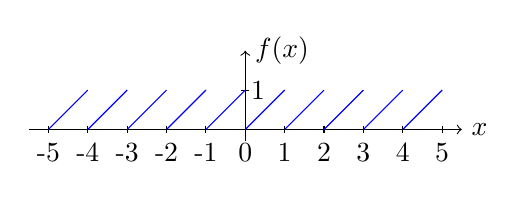
\begin{tikzpicture}[scale=0.5]
    % Axis
    \draw[->] (-5.5,0) -- (5.5,0) node[right] {\( x \)};
    \draw[->] (0,-0.3) -- (0,2) node[right] {\( f(x) \)};
    
    % Ticks
    \foreach \x in {-5,-4,...,5} {
        \draw (\x, 0.1) -- (\x, -0.1) node[below] {\x};
    }

    
    \draw (0.1, 1) -- (-0.1, 1) node[right] {1};
    
    % Function plot
    \foreach \n in {-5,-4,...,4} {
        \draw[blue] (\n, 0) -- (\n+1, 1);
    }
\end{tikzpicture}
\caption{$f(x)=x-[x]$的图像}
\label{fig:f(x)=x-[x]的图像}
\end{figure}

\item 常量函数 $f(x)=c$ 是以任何正数为周期的周期函数,但不存在基本周期.
        \end{enumerate}
\end{exercise}

\subsection{初等函数}

我们在中学接触过的基本初等函数有如表\ref{tab:基本初等函数分类表}所示的六类。它们的函数图像如图\ref{fig:basic-elem-func}所示。

\begin{table}[h]
\caption{基本初等函数分类表}
\centering
\renewcommand{\arraystretch}{1.5} % 用于增加行高
\begin{tabular}{c|c}
\hline
\rowcolor{gray!50}
\textbf{函数类型} & \textbf{函数表达式} \\
\hline
常量函数 & $y=c \quad (c$ 是常数$)$ \\
\hline
幂函数 & $y=x^u \quad (u$ 为实数$)$ \\
\hline
指数函数 & $y=a^x \quad (a>0, a \neq 1)$ \\
\hline
对数函数 & $y=\log_a x \quad (a>0, a \neq 1)$ \\
\hline
\multirow{4}{*}{三角函数} & $y=\sin x$ (正弦函数) \\
 & $y=\cos x$ (余弦函数) \\
 & $y=\tan x$ (正切函数) \\
 & $y=\cot x$ (余切函数) \\
\hline
\multirow{4}{*}{反三角函数} & $y=\arcsin x$ (反正弦函数) \\
 & $y=\arccos x$ (反余弦函数) \\
 & $y=\arctan x$ (反正切函数) \\
 & $y=\operatorname{arccot} x$ (反余切函数) \\
\hline
\end{tabular}
\label{tab:基本初等函数分类表}
\end{table}

\begin{figure}[!h]
    \centering
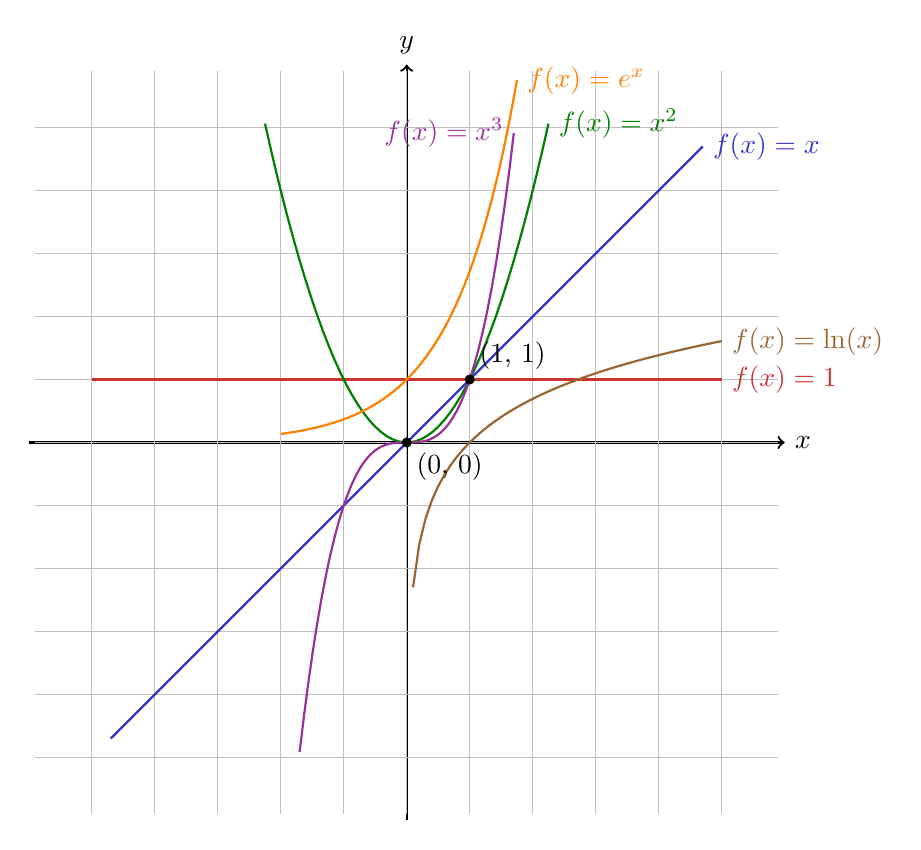
\begin{tikzpicture}[scale=0.8]

  % Draw axes
  \draw[->, thick] (-6,0) -- (6,0) node[right] {$x$};
  \draw[->, thick] (0,-6) -- (0,6) node[above] {$y$};
  
  % Draw grid
  \draw[gray!50, very thin] (-5.9,-5.9) grid[step=1cm] (5.9,5.9);
  
  % Plot constant function f(x) = 1
  \draw[myred, thick, domain=-5:5, samples=2] plot (\x, {1}) node[right] {$f(x)=1$};
  
  % Plot linear function f(x) = x
  \draw[myblue, thick, domain=-4.7:4.7, samples=2] plot (\x, {\x}) node[right] {$f(x)=x$};
  
  % Plot quadratic function f(x) = x^2
  \draw[mygreen, thick, domain=-2.25:2.25, samples=50] plot (\x, {\x*\x}) node[right] {$f(x)=x^2$};

  % Plot quadratic function f(x) = x^3
  \draw[mypurple, thick, domain=-1.7:1.7, samples=50] plot (\x, {\x*\x*\x}) node[left] {$f(x)=x^3$};
  
  % Plot exponential function f(x) = e^x
  \draw[myorange, thick, domain=-2:1.75, samples=50] plot (\x, {exp(\x)}) node[right] {$f(x)=e^x$};
  
  % Plot logarithmic function f(x) = ln(x)
  \draw[mybrown, thick, domain=0.1:5, samples=50] plot (\x, {ln(\x)}) node[right] {$f(x)=\ln(x)$};

  % Mark points
  % \filldraw [black] (1,0) circle (2pt) node[anchor=north west] {(1, 0)};
  \filldraw [black] (0,0) circle (2pt) node[anchor=north west] {(0, 0)};
  % \filldraw [black] (0,1) circle (2pt) node[anchor=north east] {(0, 1)};
  \filldraw [black] (1,1) circle (2pt) node[anchor=south west] {(1, 1)};

\end{tikzpicture}
\caption{基本初等函数的图像}
    \label{fig:basic-elem-func}
\end{figure}

幂函数 $y=x^u$ 和指数函数 $y=a^x$ 都涉及乘幂, 而在中学数 课程中只给出了有理指数乘幂的定义. 这里我们指出,无理数也可以作为幂指数。\textcolor{second}{无理指数幂和有理指数幂一起构成了实数指数幂,并保持有理指数幂的基本性质。}


\begin{definition}[初等函数]
    由基本初等函数经过\textcolor{red}{有限次四则运算与复合运算}所得到的函数, 统称为\textcolor{third}{\bf 初等函数}.
\end{definition}


\subsection{复合函数}

\subsection{反函数}

% \chapter{概率与统计}

% \textbf{这里介绍概率论的最基本内容和统计学的一些内容。计划参考gilbert书的统计部分以及实验设计教材。}

% \chapter{机器学习基础}

\printbibliography[heading=bibintoc, title=\ebibname]
\appendix

\chapter{基本数学工具}


本附录包括了计量经济学中用到的一些基本数学,我们扼要论述了求和算子的各种性质,研究了线性和某些非线性方程的性质,并复习了比例和百分数。我们还介绍了一些在应用计量经济学中常见的特殊函数,包括二次函数和自然对数,前 4 节只要求基本的代数技巧,第 5 节则对微分学进行了简要回顾;虽然要理解本书的大部分内容,微积分并非必需,但在一些章末附录和第 3 篇某些高深专题中,我们还是用到了微积分。

\section{求和算子与描述统计量}

\textbf{求和算子} 是用以表达多个数求和运算的一个缩略符号,它在统计学和计量经济学分析中扮演着重要作用。如果 $\{x_i: i=1, 2, \ldots, n\}$ 表示 $n$ 个数的一个序列,那么我们就把这 $n$ 个数的和写为:

\begin{equation}
\sum_{i=1}^n x_i \equiv x_1 + x_2 +\cdots + x_n
\end{equation}



\end{document}
